% ============================================================================
%  RESULTADOS DEL ESTUDIO PRINCIPAL — sección lista para manuscrito
% ----------------------------------------------------------------------------
%  NOTA DE PROCEDENCIA (no aparece en el PDF compilado):
%  Estadísticos de la corrida completa y verificada del pipeline
%  (Experimento ALC_v5_corregido.R, v5.9, SHA-256 1143b36a…). Origen, relativo a
%  «Analisis agosto v2/»:
%     · piloto/tablas/resumen_modelos_validos.csv            (ANOVA del modelo)
%     · principal/tablas/principal_n_palabras_calculado_EMM.csv
%     · principal/tablas/principal_n_palabras_calculado_contrastes_{tiempo,cond}.csv
%     · piloto/tablas/descriptivos_condicion_tiempo.csv      (medias y DE)
%     · resultados/tablas/datos_completos_ancho.csv          (filtrando fuente = principal)
%     · outputs/tablas/tabla_demora.csv                      (modelo con demora)
%  Figuras: copiadas de la misma corrida a la carpeta «figuras/». Las figuras de
%  contenido (temas, prototipos, emociones, similitud) disponibles se calcularon
%  sobre el CONJUNTO COMPLETO (n = 40); las de este documento son las del
%  principal o las que usan solo variables con datos en el principal.
%  Claves de cita: se conservan FuentesRibes2001, CamachoGomez2007 y Ryle2005;
%  se añade LopezCorral2024 con la entrada completa.
% ============================================================================

\documentclass[12pt]{article}
\usepackage[utf8]{inputenc}
\usepackage[T1]{fontenc}
\usepackage{lmodern}                 % fuentes vectoriales Type 1 con mapa Unicode
% rótulos de figuras y tablas en español (por defecto LaTeX usa 'Figure' y 'Table')
\renewcommand{\figurename}{Figura}
\renewcommand{\tablename}{Tabla}
\usepackage{amsmath}
\usepackage{graphicx}
\usepackage{booktabs}
\usepackage{caption}
\usepackage{subcaption}
\usepackage{geometry}
\geometry{a4paper, margin=1in}
\usepackage{setspace}
\onehalfspacing
\graphicspath{{figuras/}}

\title{Producción escrita y estímulos reactivos: resultados del estudio principal}
\author{}
\date{}

\begin{document}

\maketitle

\section{Resultados}

\subsection{Participantes, diseño y muestra analítica}

El estudio principal incluyó \textbf{23 participantes} distribuidos en tres condiciones
experimentales según el modo reactivo habilitante: Texto ($n = 8$; modo leer), Audio
($n = 8$; modo escuchar) e Imagen ($n = 7$; modo observar). Dentro de cada condición, los
participantes diferían en una segunda variable, la \emph{demora} entre la exposición al
estímulo y la escritura: en Texto, 3 con demora y 5 sin ella; en Audio, 3 y 5; en Imagen, 5 y 2.
Cada participante produjo tres textos sucesivos sobre el mismo referente (T1, sin estímulo;
T2, con un estímulo; T3, con los tres estímulos acumulados), lo que resulta en
\textbf{69 observaciones} para la variable dependiente principal.

En esta cohorte la columna \texttt{n\_palabras} del archivo de captura está completa y su
correlación con el conteo verificado sobre el texto (\texttt{n\_palabras\_calculado}) es
$\geq .999$; el análisis utilizó \texttt{n\_palabras} y los dos conteos son intercambiables
numéricamente. El estudio principal es una \textbf{muestra independiente} del estudio piloto
($n = 17$): no constituye su continuación, y las comparaciones entre ambas cohortes se tratan
como comparaciones entre muestras.

\subsection{Extensión del texto y efecto del tiempo}

La Tabla~\ref{tab:desc_principal} presenta los estadísticos descriptivos de la extensión.

\begin{table}[htbp]
	\centering
	\caption{Extensión del texto (número de palabras): media (desviación estándar) y mediana por
	condición y momento. Estudio principal, $n = 23$.}
	\label{tab:desc_principal}
	\begin{tabular}{l c c c c}
		\toprule
		Condición & Momento & $n$ & $M$ ($DE$) & Mediana \\
		\midrule
		Texto  & T1 & 8 &  88.50 (54.88) &  87.5 \\
		Texto  & T2 & 8 & 138.12 (87.38) & 129.5 \\
		Texto  & T3 & 8 & 184.62 (136.04) & 129.0 \\
		\midrule
		Audio  & T1 & 8 & 109.88 (79.51) &  89.0 \\
		Audio  & T2 & 8 & 160.88 (65.75) & 168.0 \\
		Audio  & T3 & 8 & 200.50 (66.44) & 212.0 \\
		\midrule
		Imagen & T1 & 7 &  74.43 (33.27) &  70.0 \\
		Imagen & T2 & 7 & 115.29 (66.82) & 102.0 \\
		Imagen & T3 & 7 & 155.00 (101.35) & 125.0 \\
		\bottomrule
	\end{tabular}
	\smallskip
	\emph{Nota}: la condición Texto en T3 presenta la mayor dispersión del conjunto
	($DE = 136.04$ frente a una media de 184.62), reflejo de trayectorias individuales muy
	distintas dentro del mismo grupo.
\end{table}

\begin{table}[htbp]
	\centering
	\caption{ANOVA de tipo III (Satterthwaite) del modelo mixto para el número de palabras.
	Estudio principal, 69 observaciones de 23 participantes.}
	\label{tab:anova_principal}
	\begin{tabular}{l c c c c}
		\toprule
		Efecto & $F$ & gl num. & gl den. & $p$ \\
		\midrule
		Condición                &  0.598 & 2 & 20 & .559 \\
		Tiempo                   & \textbf{25.503} & 2 & 40 & \textbf{$< .001$} \\
		Condición $\times$ tiempo &  0.075 & 4 & 40 & .989 \\
		\bottomrule
	\end{tabular}
	\smallskip
	\emph{Nota}: $R^2$ marginal $= .197$; $R^2$ condicional $= .787$. El valor exacto de
	$p$ para el efecto de tiempo es $7.24 \times 10^{-8}$.
\end{table}

El modelo mixto —efectos fijos de condición, tiempo y su interacción, con intercepto aleatorio
por participante— muestra un \textbf{efecto de tiempo claramente significativo}
($F(2,40) = 25.503$, $p < .001$) y \textbf{ningún efecto de condición}
($F(2,20) = 0.598$, $p = .559$) \textbf{ni interacción} ($F(4,40) = 0.075$, $p = .989$). La
extensión crece a lo largo del episodio y lo hace de la misma manera en las tres condiciones.
El $R^2$ marginal de .197 frente a un $R^2$ condicional de .787 indica que la mayor parte de la
variación se debe a diferencias entre participantes.

\begin{table}[htbp]
	\centering
	\caption{Medias marginales estimadas (EM), error estándar e intervalo de confianza del 95\%
	del número de palabras, por condición y momento. Estudio principal.}
	\label{tab:emm_principal}
	\begin{tabular}{l c c c c c}
		\toprule
		Condición & Momento & EM & SE & IC 95\% inf. & IC 95\% sup. \\
		\midrule
		Texto  & T1 &  88.50 & 29.03 &  29.11 & 147.90 \\
		Texto  & T2 & 138.13 & 29.03 &  78.73 & 197.52 \\
		Texto  & T3 & 184.63 & 29.03 & 125.23 & 244.02 \\
		\midrule
		Audio  & T1 & 109.87 & 29.03 &  50.48 & 169.27 \\
		Audio  & T2 & 160.87 & 29.03 & 101.48 & 220.27 \\
		Audio  & T3 & 200.50 & 29.03 & 141.11 & 259.90 \\
		\midrule
		Imagen & T1 &  74.43 & 31.04 &  10.94 & 137.92 \\
		Imagen & T2 & 115.29 & 31.04 &  51.79 & 178.79 \\
		Imagen & T3 & 155.00 & 31.04 &  91.51 & 218.49 \\
		\bottomrule
	\end{tabular}
	\smallskip
	\emph{Nota}: estimaciones con \texttt{emmeans} sobre el modelo ajustado con
	\texttt{lmerTest}; método de grados de libertad Kenward--Roger ($gl = 28.83$).
\end{table}

Los contrastes \emph{a posteriori} con ajuste de Holm (Tabla~\ref{tab:contrastes_tiempo})
precisan dónde ocurre el cambio dentro de cada condición.

\begin{table}[htbp]
	\centering
	\caption{Contrastes entre momentos dentro de cada condición (ajuste Holm) para el número de
	palabras. Estudio principal.}
	\label{tab:contrastes_tiempo}
	\begin{tabular}{l c c c c}
		\toprule
		Condición & Contraste & $\Delta$ & $t$ & $p$ \\
		\midrule
		Texto  & T1 $\to$ T2 & $-49.62$ & $-2.349$ & $.048$ \\
		Texto  & T1 $\to$ T3 & $-96.12$ & $-4.550$ & $\mathbf{< .001}$ \\
		Texto  & T2 $\to$ T3 & $-46.50$ & $-2.201$ & $.048$ \\
		\midrule
		Audio  & T1 $\to$ T2 & $-51.00$ & $-2.414$ & $.041$ \\
		Audio  & T1 $\to$ T3 & $-90.63$ & $-4.290$ & $\mathbf{< .001}$ \\
		Audio  & T2 $\to$ T3 & $-39.63$ & $-1.876$ & $.068$ \\
		\midrule
		Imagen & T1 $\to$ T2 & $-40.86$ & $-1.809$ & $.156$ \\
		Imagen & T1 $\to$ T3 & $-80.57$ & $-3.568$ & $\mathbf{.003}$ \\
		Imagen & T2 $\to$ T3 & $-39.71$ & $-1.759$ & $.156$ \\
		\bottomrule
	\end{tabular}
	\smallskip
	\emph{Nota}: los signos negativos indican incremento de palabras en la dirección del
	contraste. El valor exacto de $p$ para Texto T1$\to$T3 es $1.47 \times 10^{-4}$ y para
	Audio T1$\to$T3, $3.30 \times 10^{-4}$.
\end{table}

El incremento acumulado de T1 a T3 es significativo en las tres condiciones
($\Delta$ entre 80.57 y 96.12 palabras). La diferencia entre condiciones es, en cambio,
inexistente en todos los momentos: ninguno de los nueve contrastes entre condiciones alcanzó
significación (todos los $p$ entre $.877$ y $1.000$; el mayor fue Audio$-$Imagen en T3,
$\Delta = 45.50$, $p = .880$). En otras palabras, \textbf{todas las condiciones crecen y crecen
igual}.

\subsection{Estructura del texto}

El análisis no se limitó al número de palabras. Se ajustaron los mismos modelos mixtos a cuatro
medidas adicionales de estructura (Tabla~\ref{tab:estructura}).

\begin{table}[htbp]
	\centering
	\caption{Modelos mixtos para las medidas de estructura del texto. Estudio principal.}
	\label{tab:estructura}
	\small
	\begin{tabular}{l c c c c}
		\toprule
		Medida & $F$ tiempo & $p$ tiempo & $p$ condición & $p$ interacción \\
		\midrule
		Número de tokens (palabras con contenido) & 26.051 & $\mathbf{< .001}$ & .580 & .989 \\
		Número de oraciones & 11.078 & $\mathbf{< .001}$ & .983 & .789 \\
		Palabras por oración & 3.082 & .057 & .598 & .210 \\
		Longitud media de palabra & 0.230 & .796 & .293 & .051 \\
		\bottomrule
	\end{tabular}
	\smallskip
	\emph{Nota}: 69 observaciones de 23 participantes en cada modelo. $p$ de tiempo exacto:
	$5.70 \times 10^{-8}$ para tokens y $1.49 \times 10^{-4}$ para oraciones. $R^2$ condicional
	entre .625 y .859.
\end{table}

El crecimiento del texto es en palabras y en oraciones, no en complejidad sintáctica por
oración: mientras el número de tokens ($F(2,40) = 26.05$, $p < .001$) y el de oraciones
($F(2,40) = 11.08$, $p < .001$) crecen con el tiempo, la razón palabras por oración
($p = .057$) y la longitud media de las palabras ($p = .796$) se mantienen estables.

\subsection{Diversidad léxica}

El Type-Token Ratio (TTR) descendió a lo largo del episodio en las tres condiciones
(Texto: $0.86 \to 0.78 \to 0.75$; Audio: $0.84 \to 0.81 \to 0.79$; Imagen:
$0.87 \to 0.84 \to 0.81$). El modelo mixto mostró un efecto de tiempo significativo
($F(2,40) = 10.27$, $p < .001$, $p$ exacto $= 2.52 \times 10^{-4}$), sin efecto de condición
($p = .663$) ni interacción ($p = .471$; $R^2$ marginal $= .113$, $R^2$ condicional $= .763$).

Este resultado debe leerse con una precaución conocida: el TTR es sensible a la longitud del
texto, y aquí los textos crecieron de forma marcada. El descenso del TTR es, por tanto,
compatible con dos explicaciones que estos datos no separan: (i) que al escribir más se
recurra a vocabulario más repetido, o (ii) que el propio indicador descienda por el aumento de
la extensión. La comparación con el estudio piloto resulta informativa en este punto: allí,
donde el efecto general de tiempo sobre la extensión \emph{no} se observó, el TTR tampoco
descendió ($p = .144$). Los dos indicadores se mueven juntos, lo que apoya la segunda
explicación y aconseja no interpretar el TTR como un índice de riqueza independiente de la
extensión.

\subsection{El papel de la demora}

La demora entre la exposición al estímulo y la escritura se evaluó añadiéndola como efecto
fijo al modelo (Tabla~\ref{tab:demora}).

\begin{table}[htbp]
	\centering
	\caption{Modelo mixto con demora añadida como efecto fijo. Estudio principal, $n = 23$.}
	\label{tab:demora}
	\begin{tabular}{l c c c c}
		\toprule
		Efecto & $F$ & gl num. & gl den. & $p$ \\
		\midrule
		Condición                 & 0.654 & 2 & 19 & .531 \\
		Tiempo                    & \textbf{25.503} & 2 & 40 & \textbf{$< .001$} \\
		Demora                    & 0.171 & 1 & 19 & .684 \\
		Condición $\times$ tiempo  & 0.075 & 4 & 40 & .989 \\
		\bottomrule
	\end{tabular}
	\smallskip
	\emph{Nota}: $R^2$ marginal $= .196$; $R^2$ condicional $= .794$. Medias marginales por
	demora: con demora $M = 143.4$ (IC 95\% $[94.5, 192.3]$), sin demora $M = 129.6$
	(IC 95\% $[81.9, 177.3]$).
\end{table}

La demora no mostró efecto ($F(1,19) = 0.171$, $p = .684$) y su inclusión no modificó ni el
efecto de tiempo ($F$ idéntico) ni la interacción. Con grupos de 3 a 5 participantes por celda y
un diseño no balanceado, este resultado no debe leerse como ausencia de efecto, sino como
ausencia de evidencia de efecto en este análisis: la potencia para detectar un efecto moderado
de la demora es muy baja.

\subsection{Estabilidad semántica entre segmentos}

La similitud coseno entre los vectores de los tres textos de cada participante
(\texttt{paraphrase-multilingual-MiniLM-L12-v2}) fue mayor entre el segundo y el tercer texto
($M = 0.928$, $DE = 0.131$) que entre el primero y el segundo ($M = 0.898$, $DE = 0.140$) y que
entre el primero y el tercero ($M = 0.866$, $DE = 0.166$). El modelo mixto con el par de
comparación como único efecto fijo fue significativo ($F(2,44) = 5.898$, $p = .005$).

El patrón reproduce, en la cohorte principal, el que se observó en el piloto: el cambio menor
ocurre entre los dos últimos textos, es decir, una vez que el escritor ya dispone de una versión
escrita del referente. Los valores absolutos son más altos que en el piloto en los tres pares,
lo que sugiere textos más homogéneos entre sí en esta muestra.

\subsection{Contenido: temas y prototipos (análisis exploratorio)}

Las tasas por 1000 palabras de los diez diccionarios temáticos aparecen en la
Tabla~\ref{tab:temas_principal}, y los cambios de proximidad a prototipos entre T1 y T3, en la
Tabla~\ref{tab:prototipos_principal}.

\begin{table}[htbp]
	\centering
	\caption{Tasas por 1000 palabras de los diccionarios temáticos, por momento. Estudio
	principal ($n = 23$).}
	\label{tab:temas_principal}
	\begin{tabular}{l c c c}
		\toprule
		Tema & T1 & T2 & T3 \\
		\midrule
		Espacio             & 31.19 & 25.71 & 25.03 \\
		Soledad             & 29.88 & 23.48 & 18.25 \\
		Objetos             & 26.92 & 25.69 & 24.55 \\
		Pasividad           &  3.91 &  2.25 &  1.59 \\
		Incomunicación      &  3.73 &  2.06 &  2.28 \\
		Emociones negativas &  1.80 &  3.27 &  2.09 \\
		Luz y sombra        &  0.23 &  1.26 &  2.33 \\
		Espera              &  0.00 &  0.68 &  1.30 \\
		Duda                &  0.56 &  0.37 &  0.98 \\
		Desconexión         &  0.00 &  0.18 &  0.00 \\
		\bottomrule
	\end{tabular}
	\smallskip
	\emph{Nota}: las desviaciones estándar son iguales o mayores que las medias en casi todas
	las celdas. Los diccionarios de \emph{desconexión} y \emph{incomunicación} apenas registran
	actividad; en el caso de desconexión, la tasa es prácticamente cero en los tres momentos.
\end{table}

\begin{table}[htbp]
	\centering
	\caption{Cambios en la proximidad a prototipos semánticos de T1 a T3 (diez mayores en valor
	absoluto). Estudio principal ($n = 23$).}
	\label{tab:prototipos_principal}
	\begin{tabular}{l c c c}
		\toprule
		Prototipo & $\Delta$ medio & $DE$ & Mediana \\
		\midrule
		Agencia             & $+0.026$ & 0.067 & $+0.021$ \\
		Duda                & $+0.023$ & 0.051 & $+0.003$ \\
		Soledad             & $-0.020$ & 0.083 & $+0.002$ \\
		Pasividad           & $-0.020$ & 0.058 & $-0.006$ \\
		Esperanza           & $+0.019$ & 0.053 & $+0.011$ \\
		Luz y sombra        & $+0.017$ & 0.096 & $+0.008$ \\
		Control             & $+0.014$ & 0.042 & $+0.011$ \\
		Confianza           & $+0.013$ & 0.032 & $+0.006$ \\
		Emociones negativas & $+0.013$ & 0.059 & $+0.016$ \\
		Miedo               & $+0.013$ & 0.047 & $+0.015$ \\
		\bottomrule
	\end{tabular}
	\smallskip
	\emph{Nota}: en todos los constructos la desviación estándar supera a la media. Estos
	análisis (20 constructos y 10 temas) no recibieron corrección por comparaciones múltiples ni
	prueba inferencial, por lo que se reportan como \textbf{exploratorios}.
\end{table}

Los patrones descriptivos son pequeños y heterogéneos: las tasas de soledad y espacio
descienden a lo largo del episodio, la de luz y sombra aumenta, y los cambios de proximidad a
prototipos rara vez superan $|0.026|$ con dispersiones mayores que la media. En conjunto, estos
datos \textbf{no sostienen} una afirmación de desplazamiento temático o emocional sistemático.

\subsection{Figuras}

\begin{figure}[htbp]
	\centering
	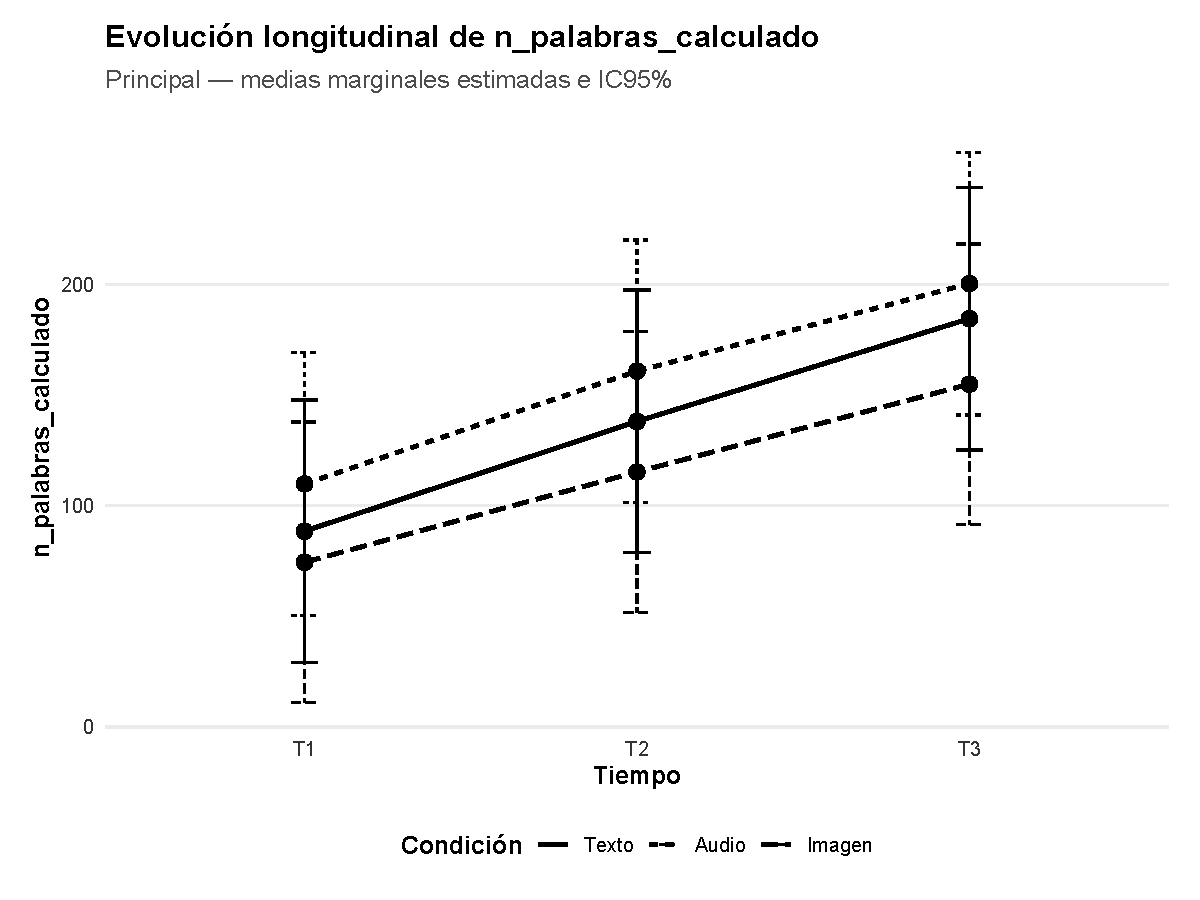
\includegraphics[width=0.95\textwidth]{PRINCIPAL_n_palabras_calculado_ES_trayectoria.pdf}
	\caption{Trayectoria de la extensión del texto por condición. Medias marginales estimadas del
	modelo mixto con intervalos de confianza del 95\%. Estudio principal ($n = 23$). Las tres
	condiciones parten de niveles distintos y crecen en paralelo: la ausencia de interacción
	($p = .989$) se ve como trayectorias sin cruce ni convergencia diferencial.}
	\label{fig:principal_trayectoria}
\end{figure}

\begin{figure}[htbp]
	\centering
	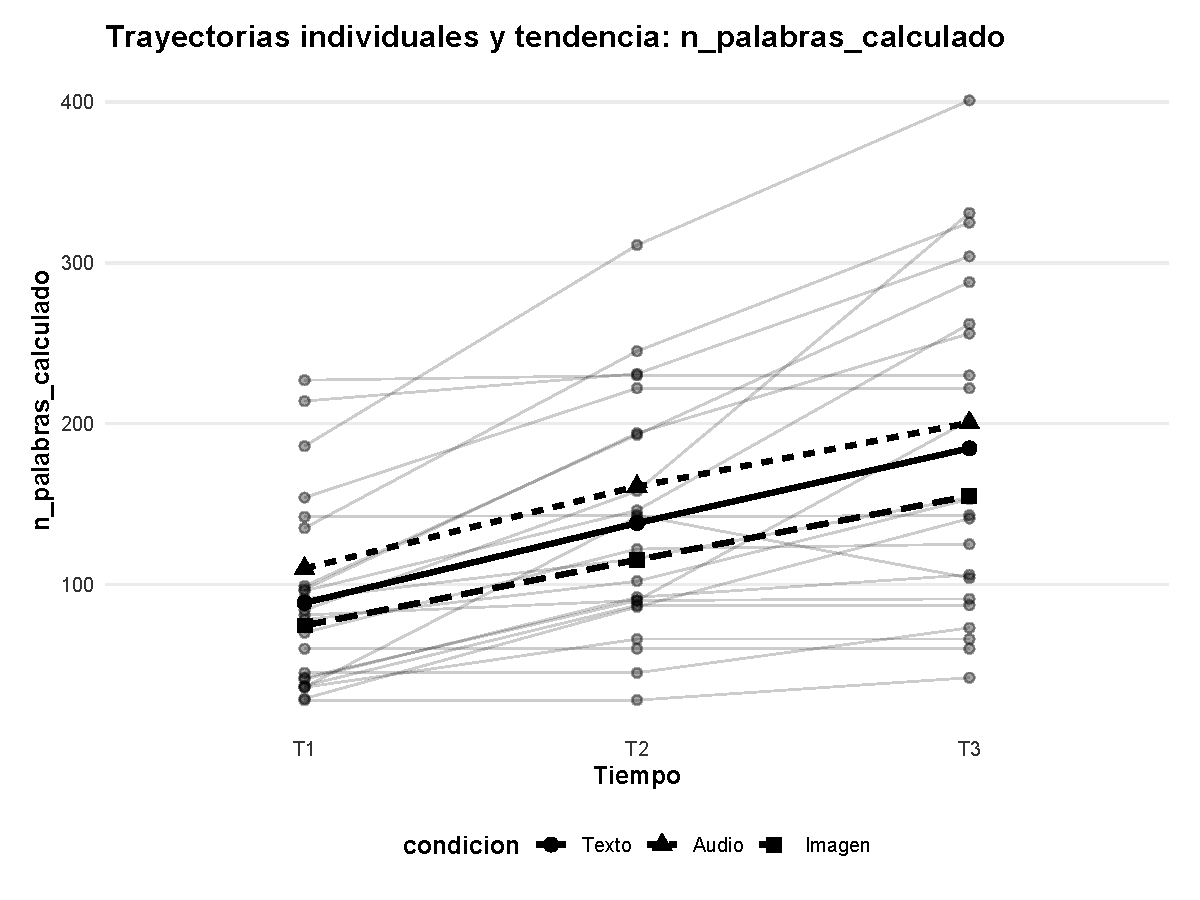
\includegraphics[width=0.95\textwidth]{PRINCIPAL_n_palabras_calculado_ES_individuales.pdf}
	\caption{Trayectorias individuales (líneas finas) y tendencia grupal (línea gruesa) de la
	extensión del texto, por condición. Estudio principal ($n = 23$). El abanico de las líneas
	individuales —especialmente en la condición Texto— muestra por qué el $R^2$ condicional
	($.787$) es alto y el marginal bajo: la variación entre personas domina la variación
	atribuible a la condición y al momento.}
	\label{fig:principal_individuales}
\end{figure}

\begin{figure}[htbp]
	\centering
	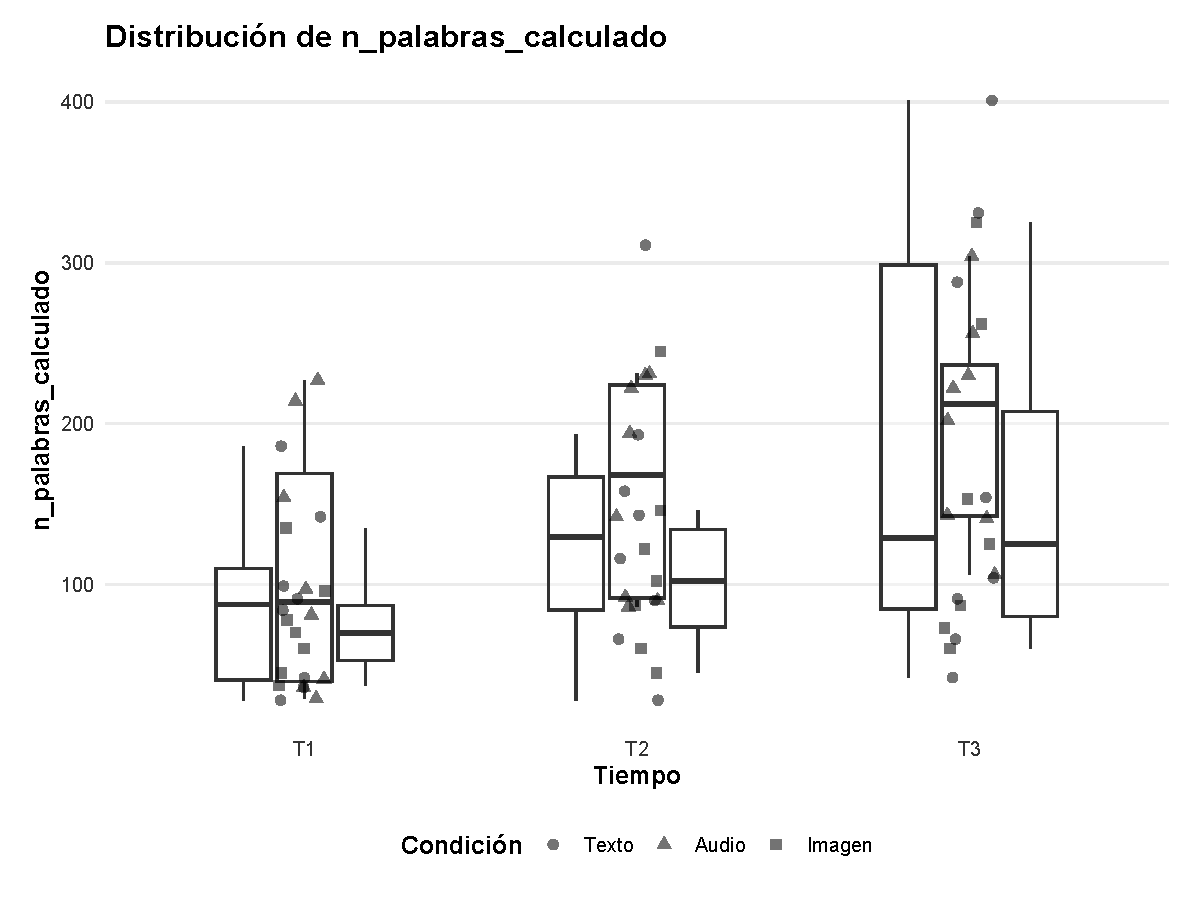
\includegraphics[width=0.95\textwidth]{PRINCIPAL_n_palabras_calculado_ES_distribucion.pdf}
	\caption{Distribución del número de palabras por condición y momento (diagramas de caja con
	observaciones individuales). Estudio principal ($n = 23$). La asimetría y la amplitud de las
	cajas en T3 explican que las medias marginales tengan intervalos de confianza amplios pese al
	efecto de tiempo robusto.}
	\label{fig:principal_distribucion}
\end{figure}

\begin{figure}[htbp]
	\centering
	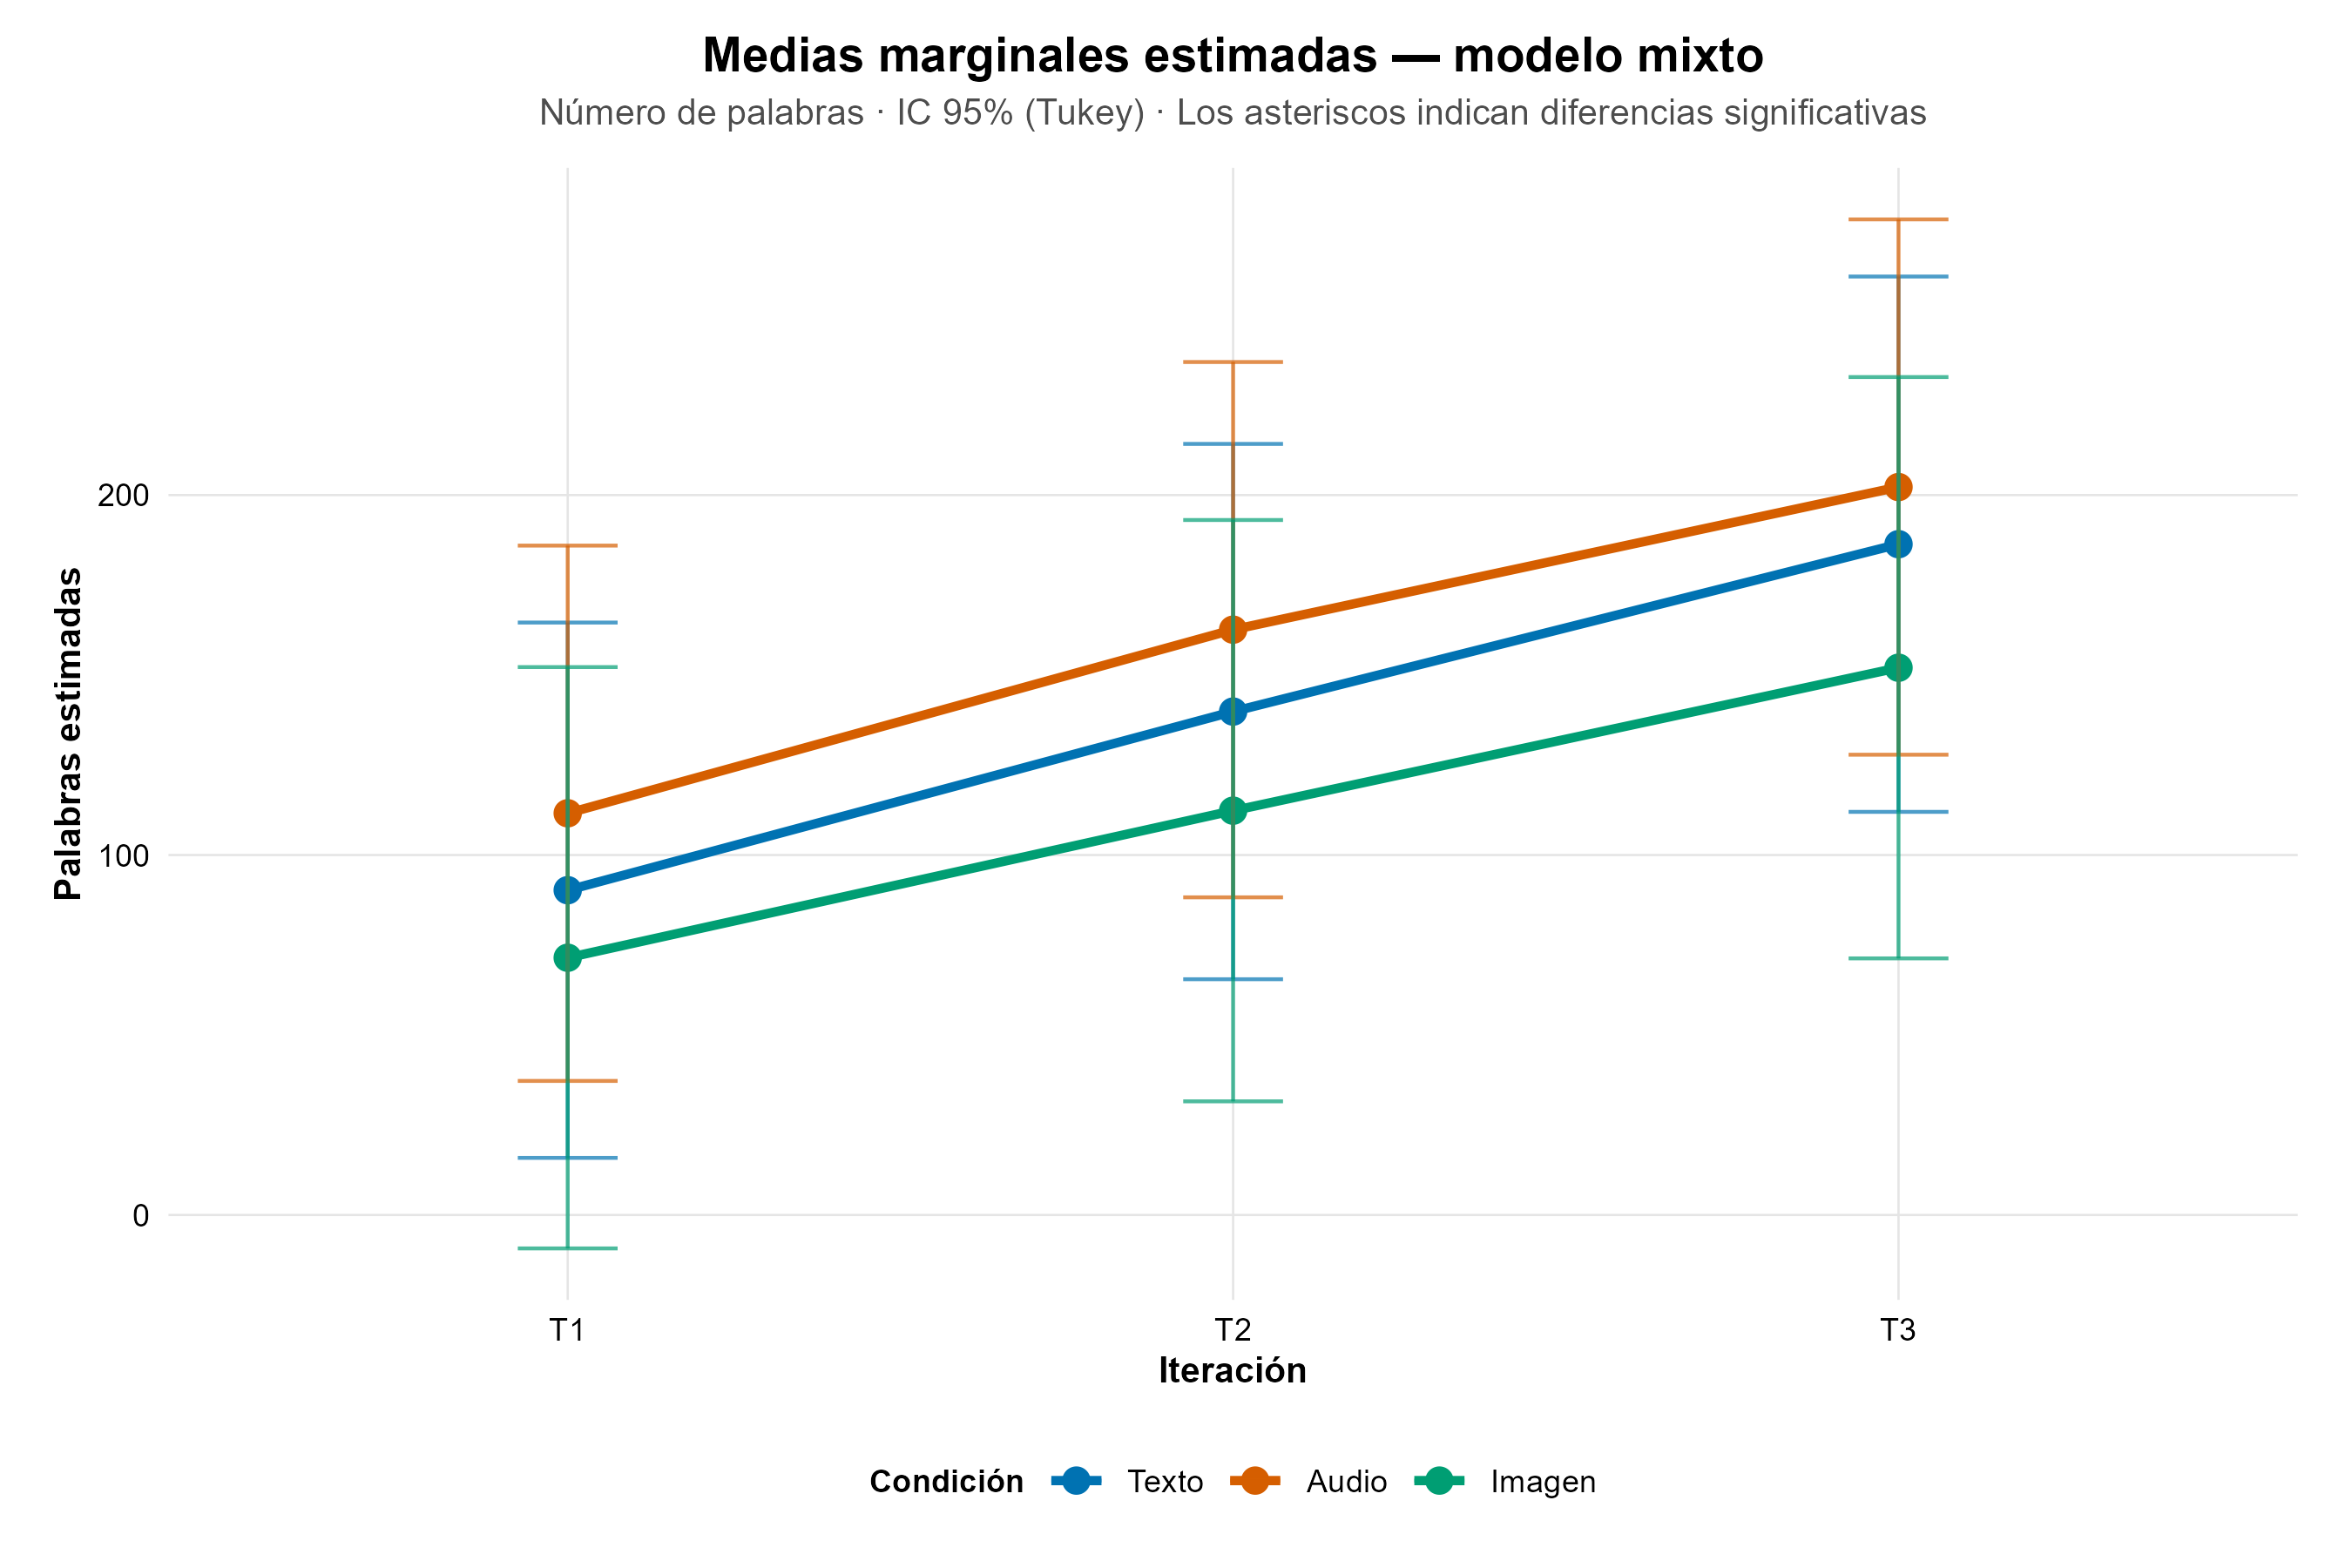
\includegraphics[width=0.95\textwidth]{fig5_modelo_estimado.png}
	\caption{Medias marginales estimadas del modelo mixto de número de palabras, con intervalos
	de confianza del 95\%. Estudio principal. Es la misma información que la
	Figura~\ref{fig:principal_trayectoria} en la presentación del script de análisis, útil para
	comprobar que ambos procedimientos coinciden.}
	\label{fig:principal_emm}
\end{figure}

\begin{figure}[htbp]
	\centering
	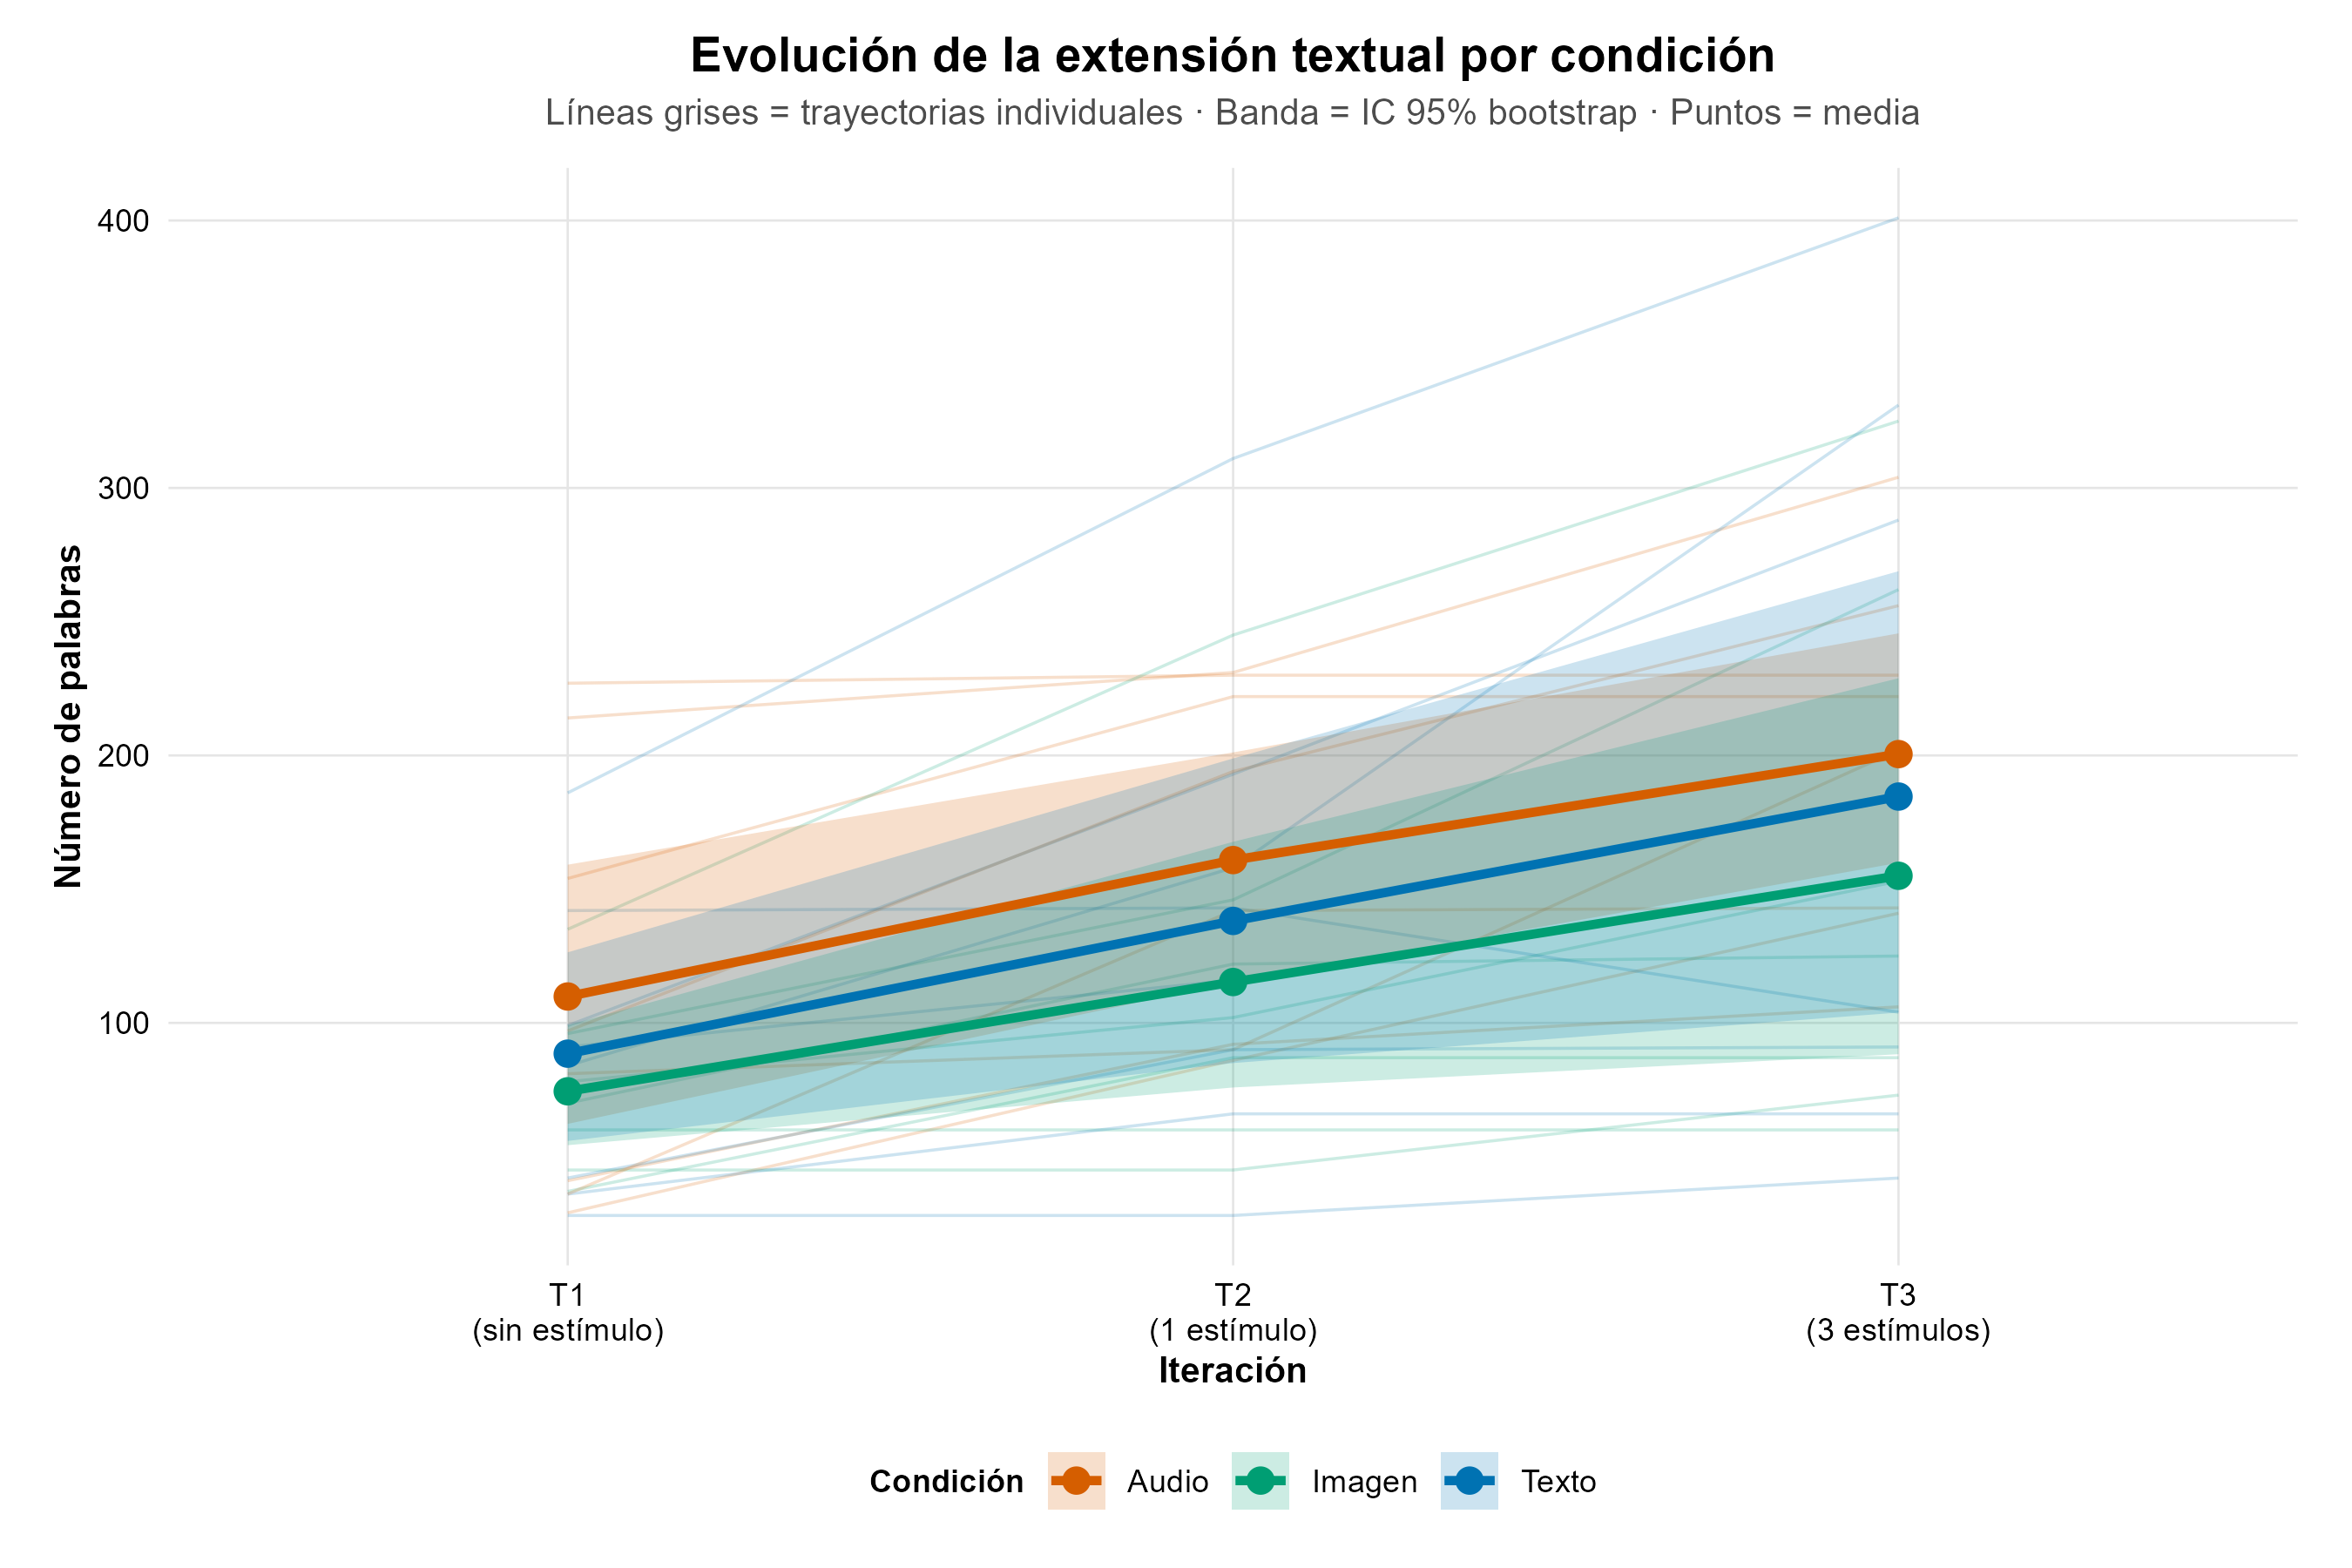
\includegraphics[width=0.95\textwidth]{fig1_palabras_condicion.png}
	\caption{Evolución de la extensión textual por condición. Líneas grises: trayectorias
	individuales; banda: intervalo de confianza del 95\% por bootstrap; puntos: media. La figura
	usa la columna \texttt{n\_palabras}, disponible únicamente en el estudio principal, de modo
	que representa a los 23 participantes de esta cohorte.}
	\label{fig:principal_fig1}
\end{figure}

\begin{figure}[htbp]
	\centering
	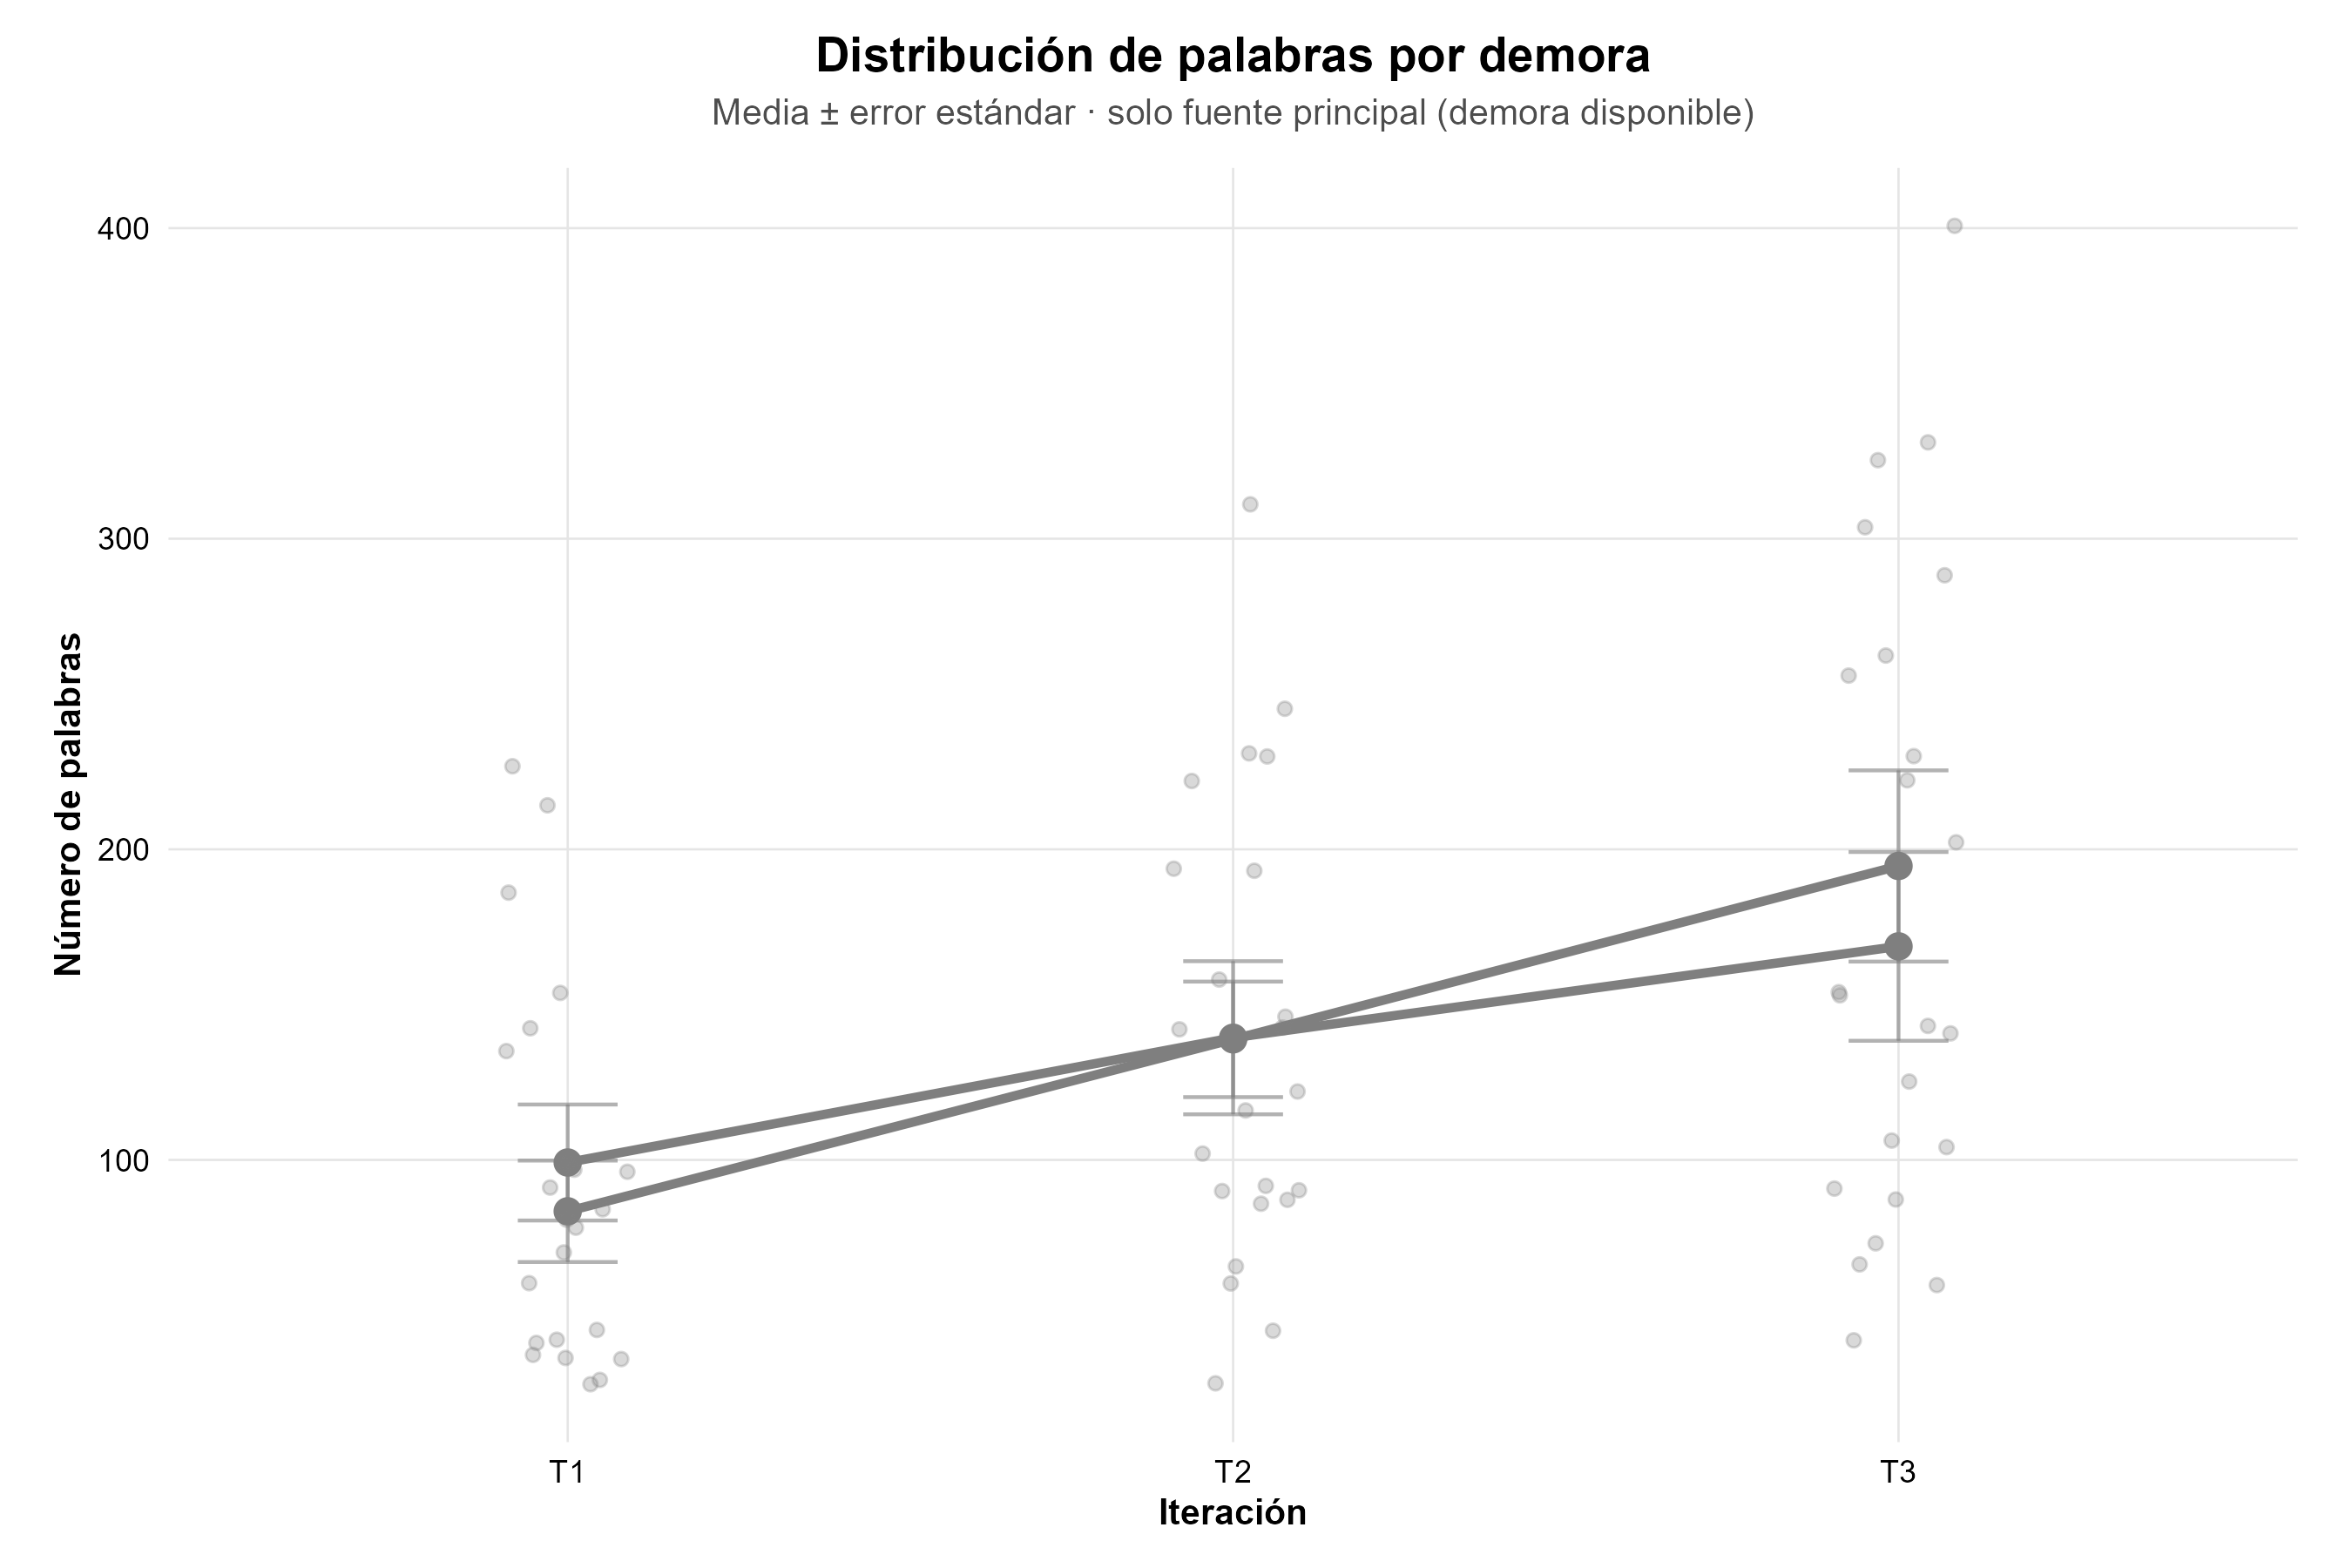
\includegraphics[width=0.95\textwidth]{fig2_palabras_demora.png}
	\caption{Extensión del texto por condición de demora (media $\pm$ error estándar, con
	observaciones individuales). Estudio principal. La figura ilustra el resultado de la
	Tabla~\ref{tab:demora}: las dos condiciones de demora siguen trayectorias paralelas, sin
	efecto detectables en el modelo.}
	\label{fig:principal_demora}
\end{figure}

\begin{figure}[htbp]
	\centering
	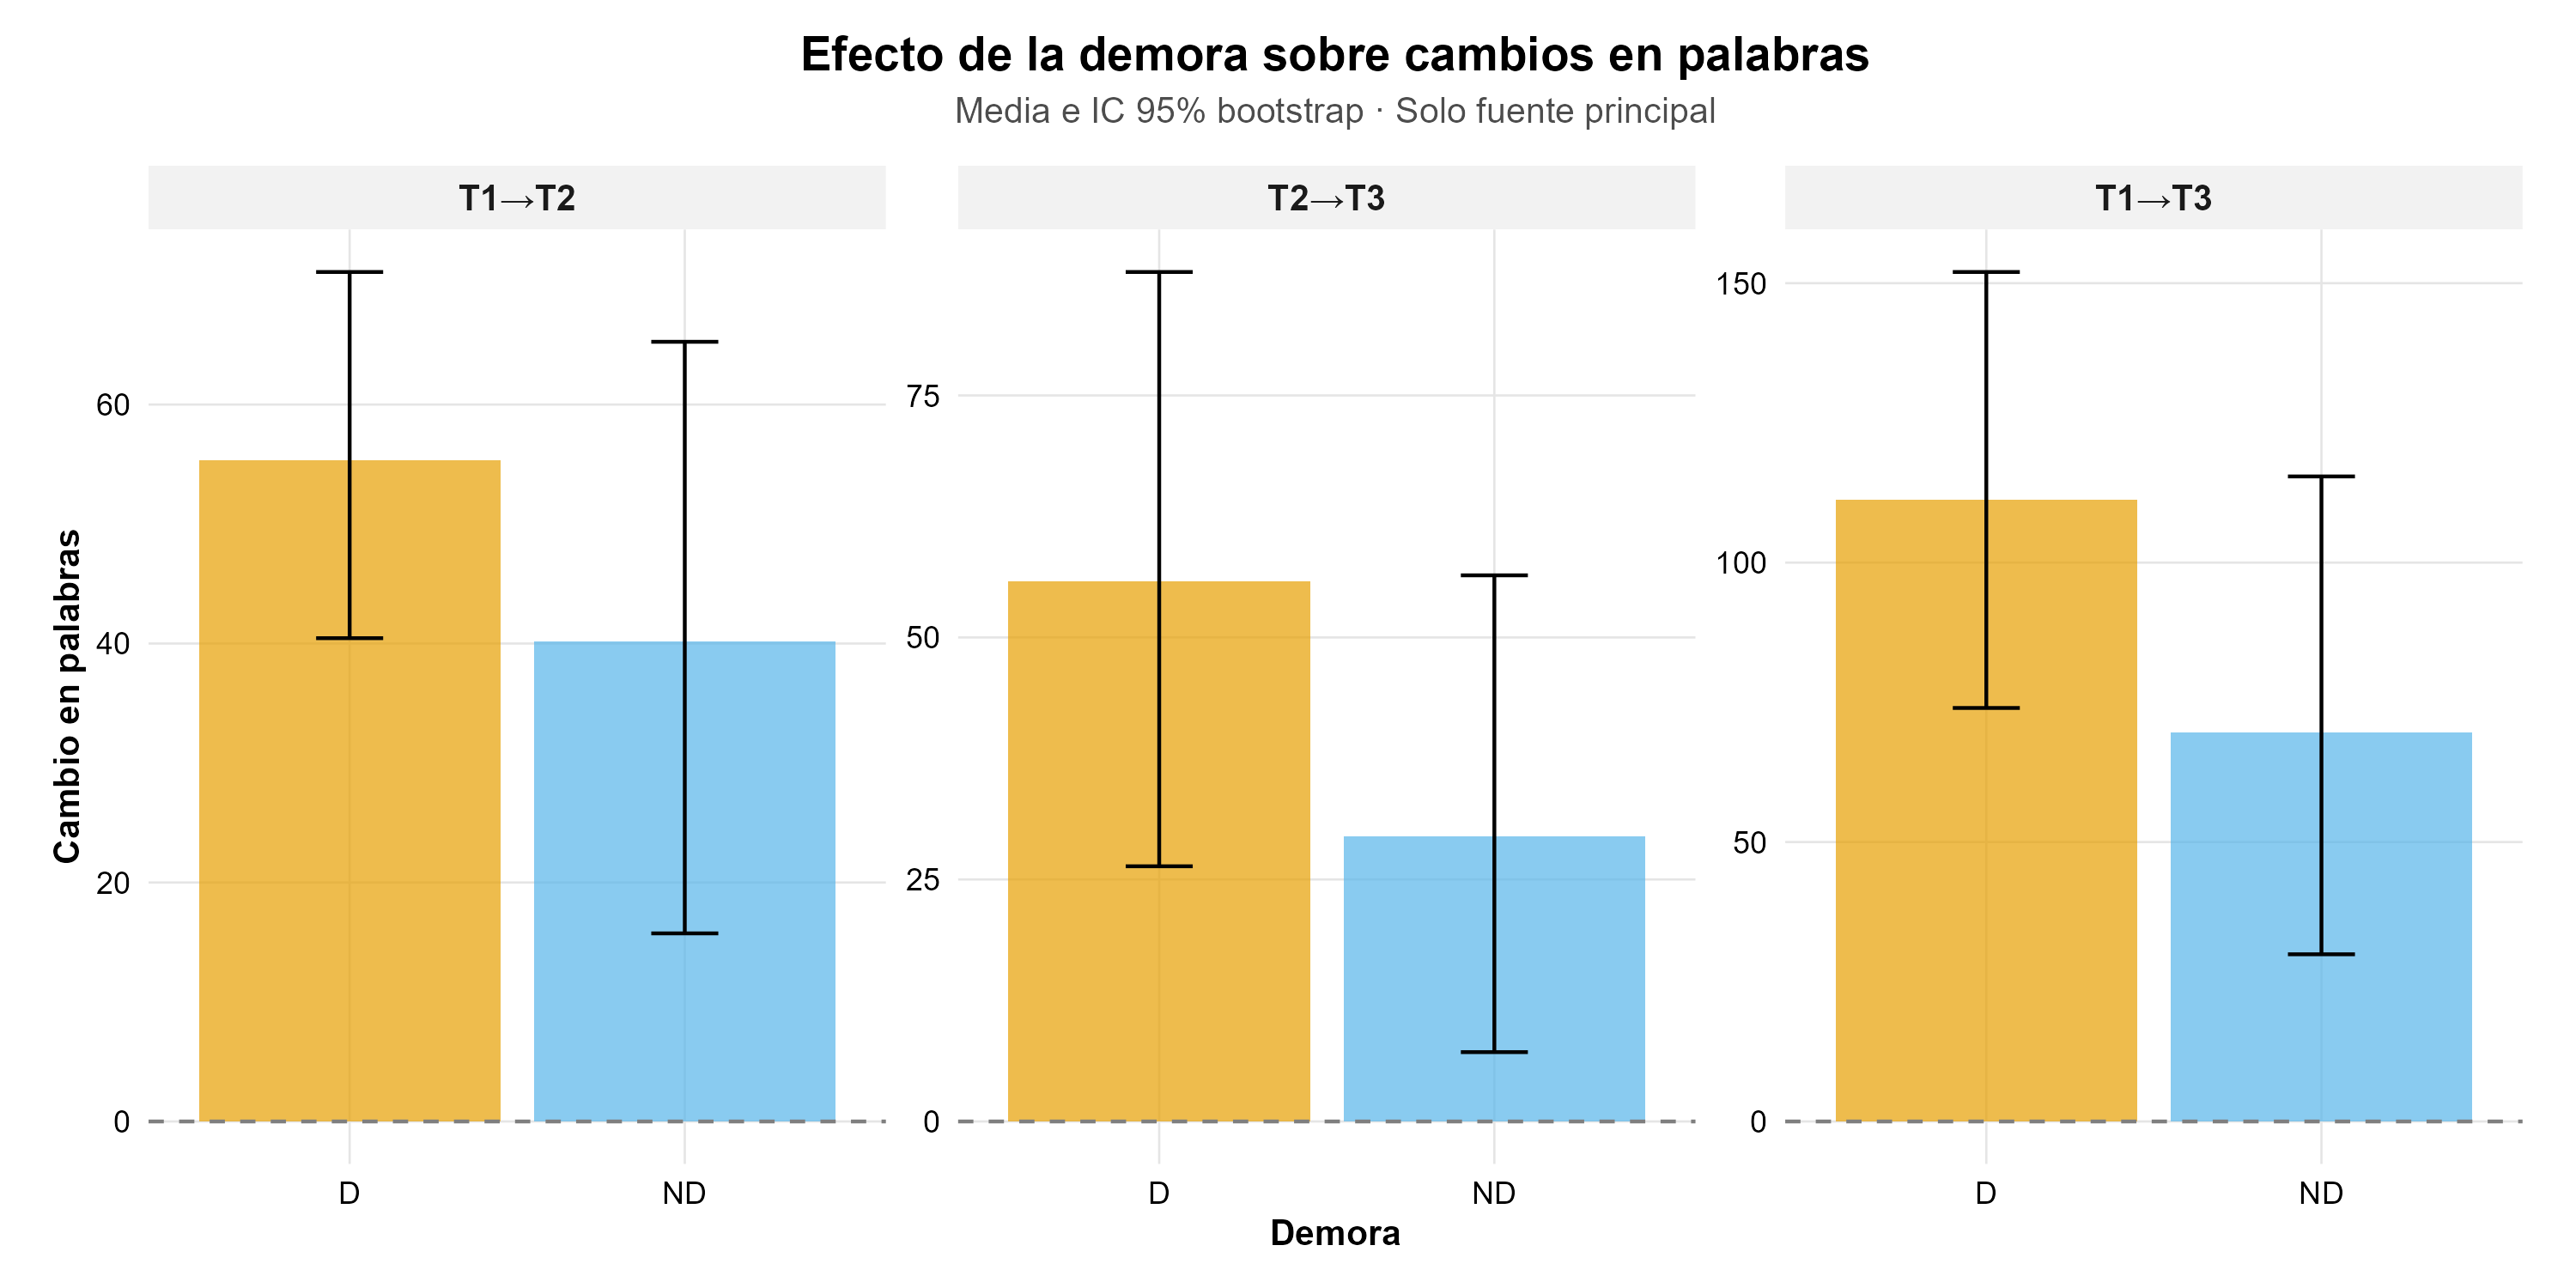
\includegraphics[width=0.95\textwidth]{fig11_efecto_demora.png}
	\caption{Cambio medio en el número de palabras (T1$\to$T2, T2$\to$T3 y T1$\to$T3) por
	condición de demora, con intervalos de confianza por bootstrap. Estudio principal. Los
	intervalos se solapan en los tres contrastes, en línea con la ausencia de efecto de demora.}
	\label{fig:principal_demora_cambios}
\end{figure}

\begin{figure}[htbp]
	\centering
	\begin{subfigure}{0.32\textwidth}
		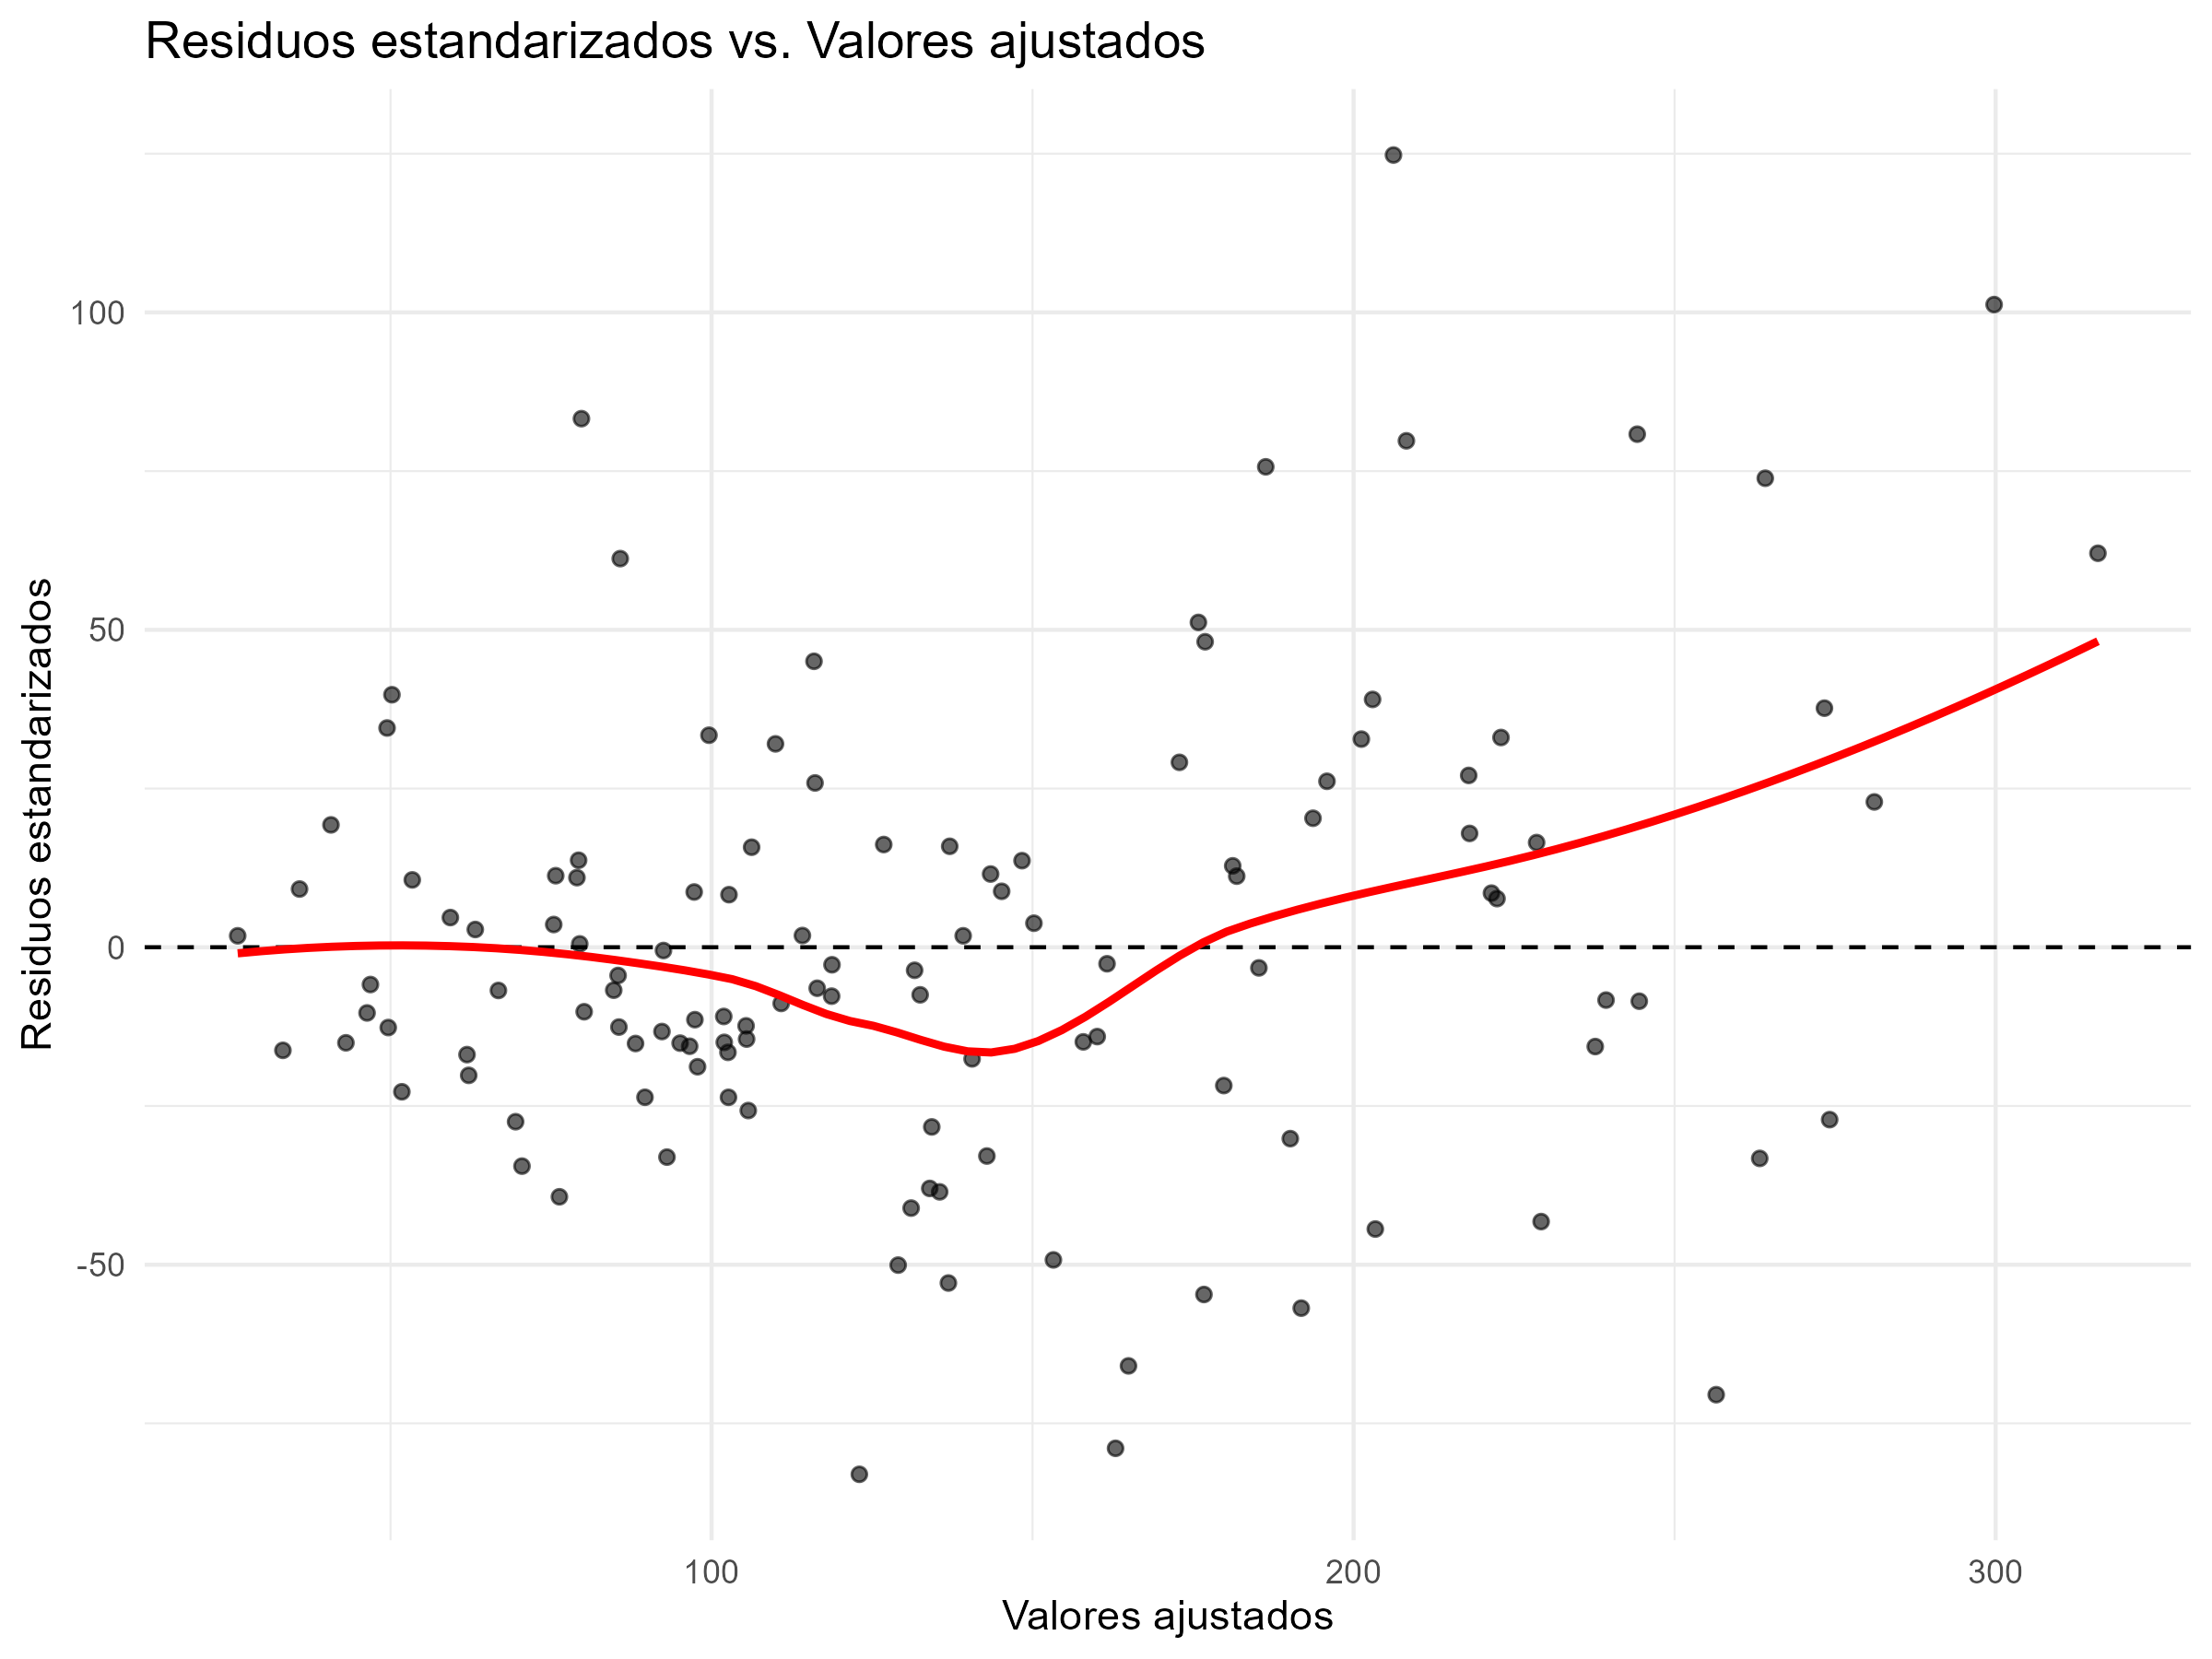
\includegraphics[width=\textwidth]{residuos_vs_ajustados.png}
		\caption{Residuos vs. ajustados}
	\end{subfigure}
	\hfill
	\begin{subfigure}{0.32\textwidth}
		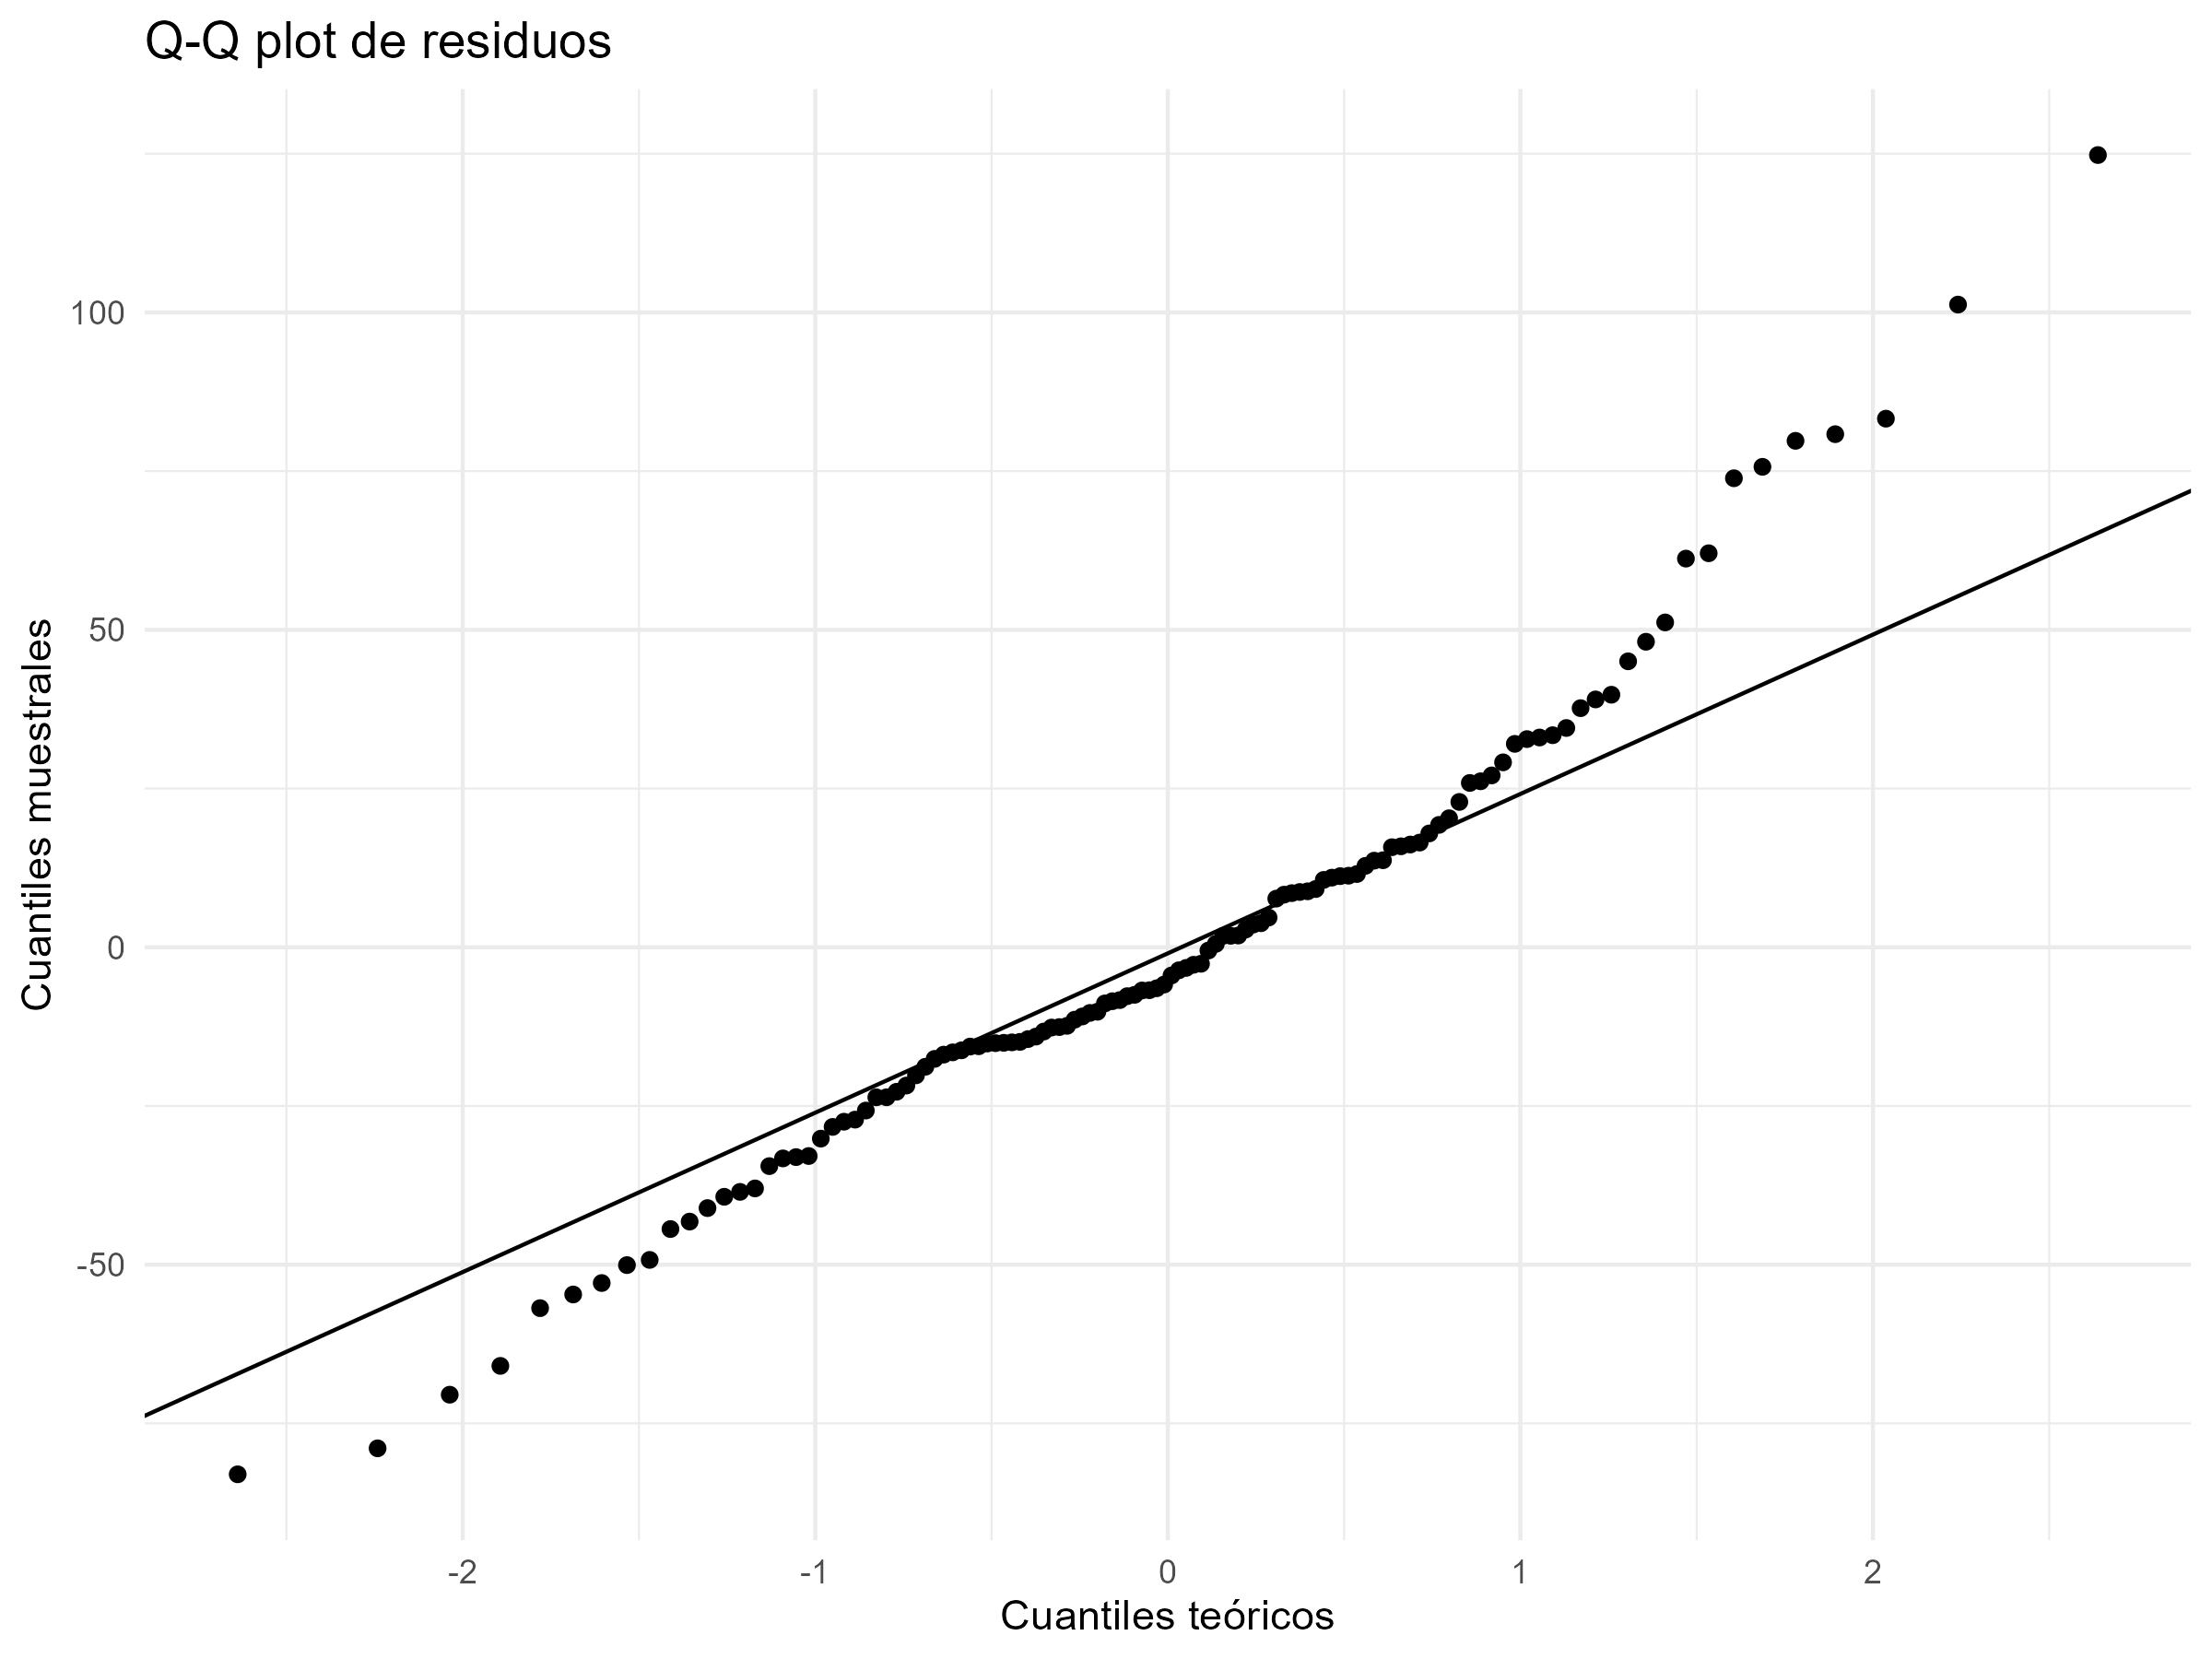
\includegraphics[width=\textwidth]{qq_residuos.png}
		\caption{Q--Q de residuos}
	\end{subfigure}
	\hfill
	\begin{subfigure}{0.32\textwidth}
		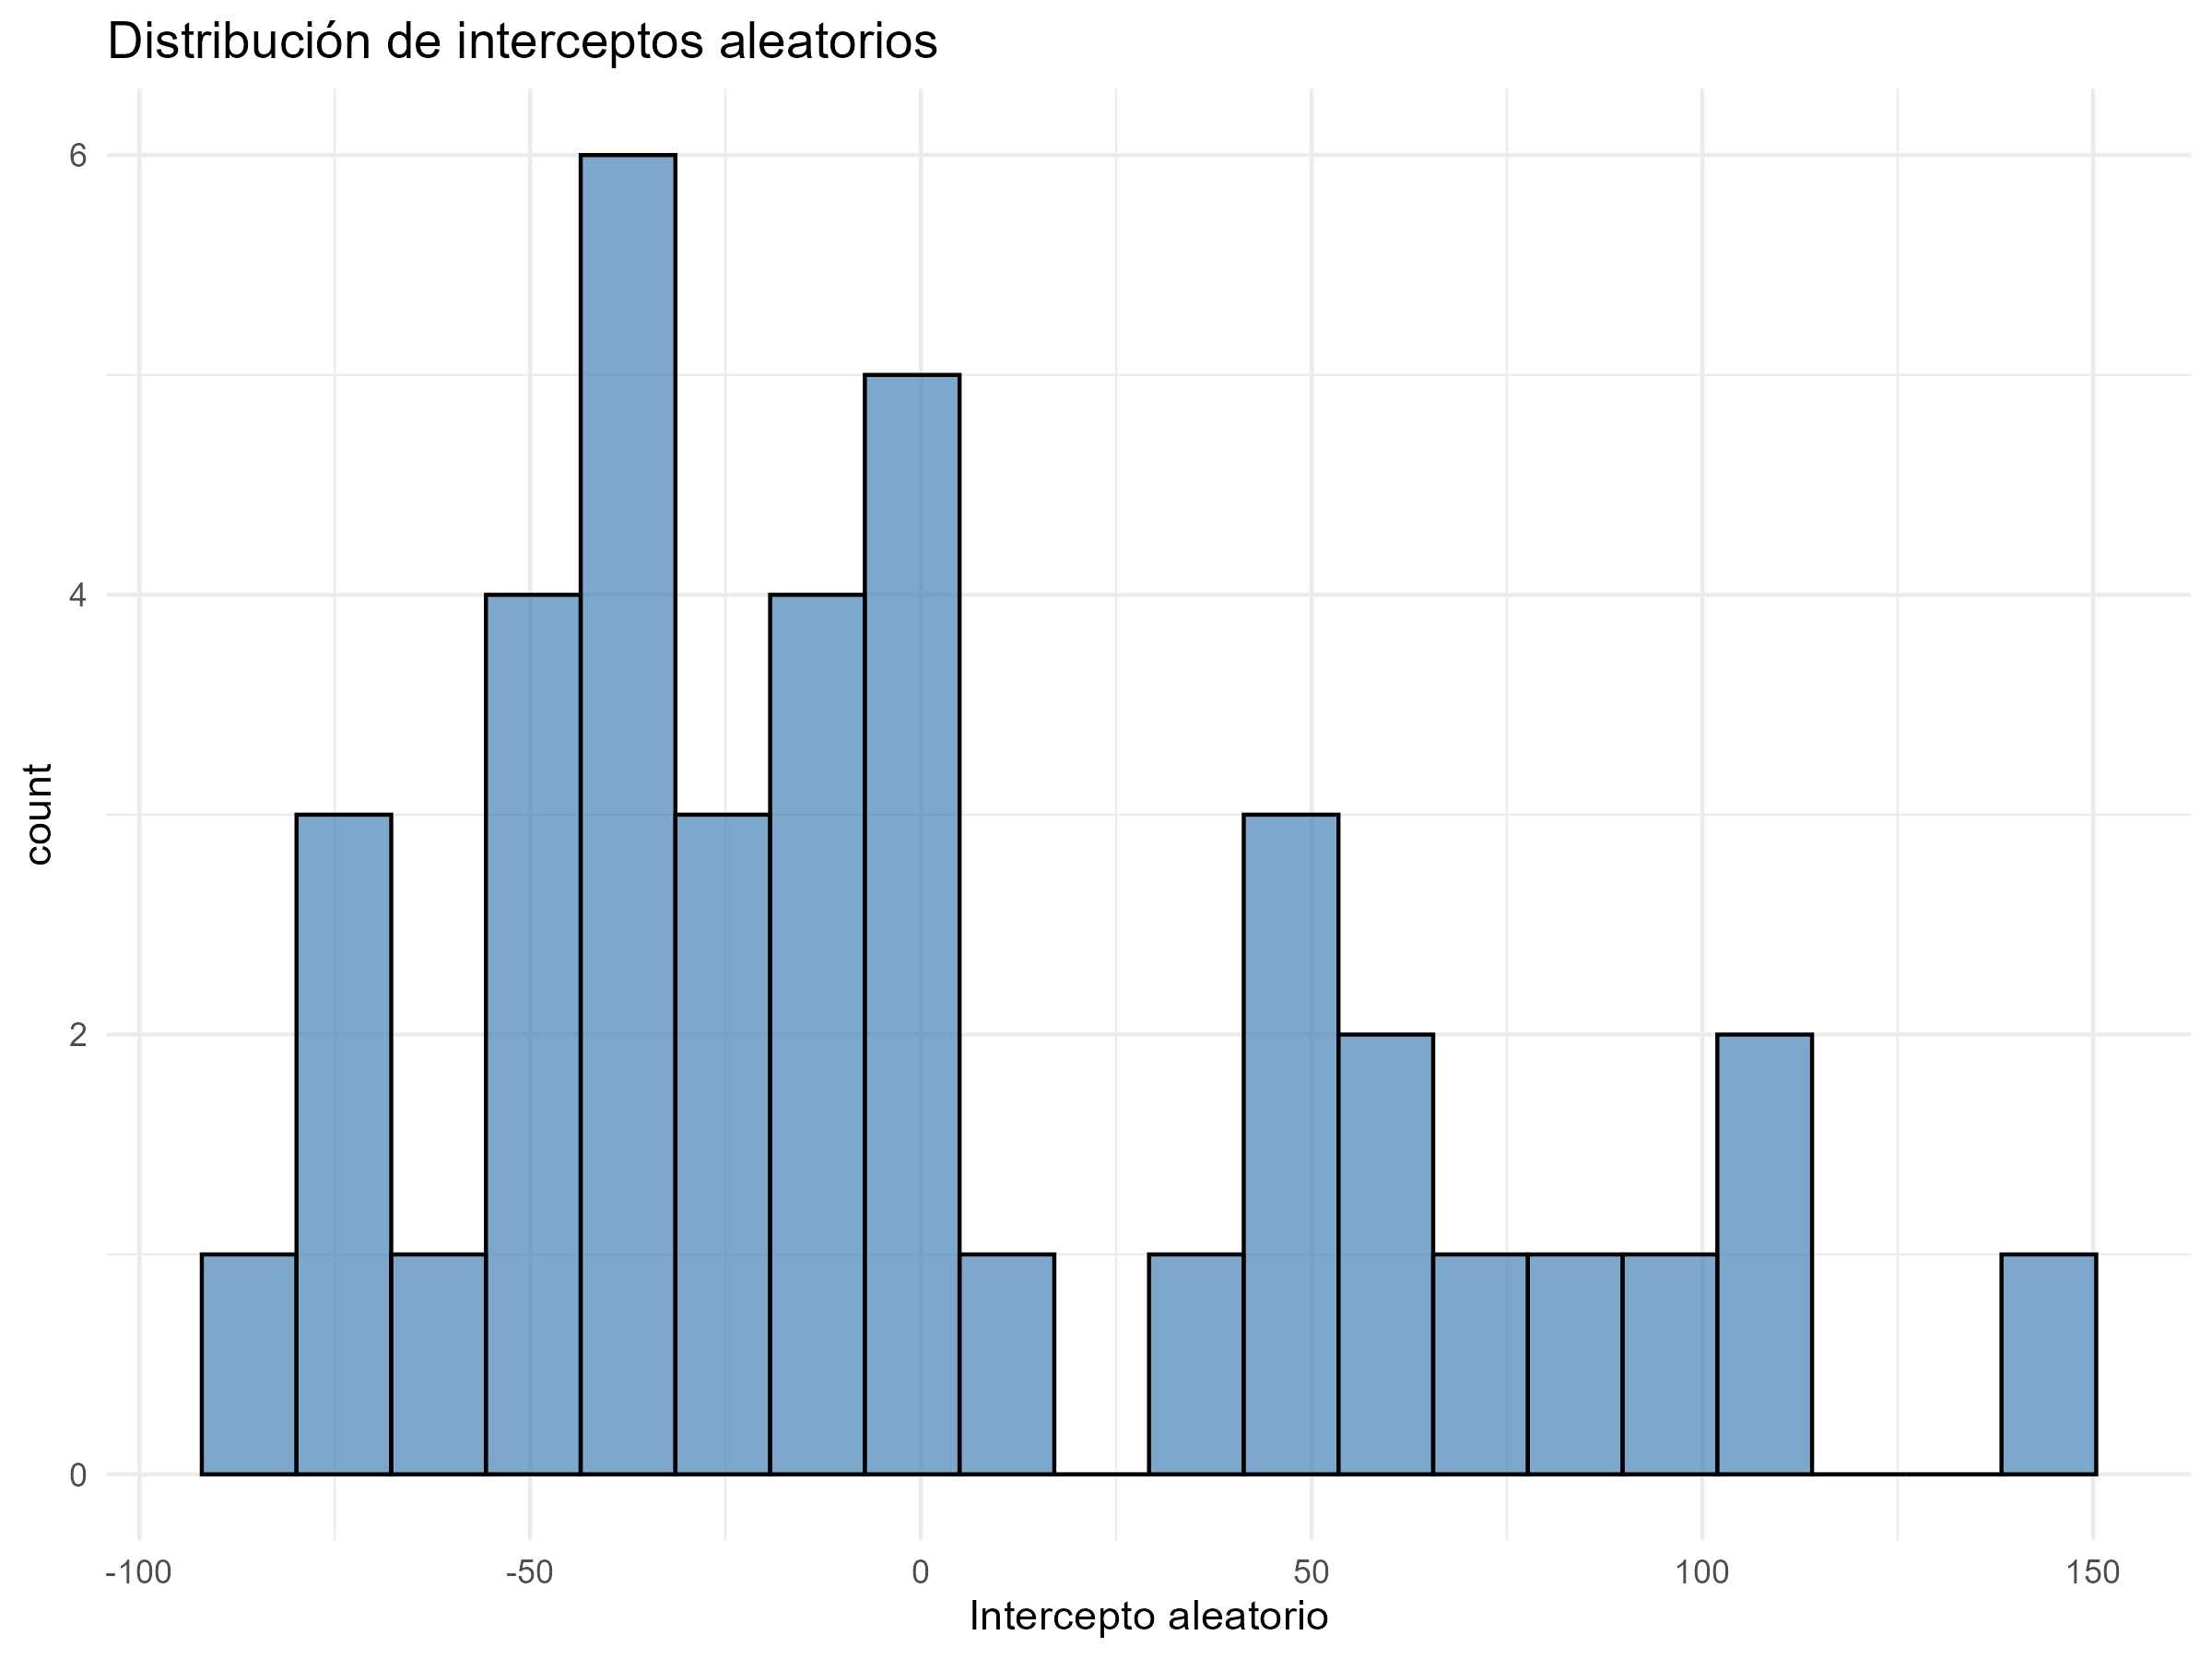
\includegraphics[width=\textwidth]{distribucion_aleatorios.png}
		\caption{Interceptos aleatorios}
	\end{subfigure}
	\caption{Diagnósticos del modelo mixto principal. Estudio principal, 69 observaciones de 23
	participantes. (a) La nube de residuos no muestra estructura frente a los valores ajustados;
	(b) la cola superior del gráfico Q--Q se separa de la recta, lo que indica residuos más
	extremos que los de una normal; (c) la distribución de interceptos aleatorios es amplia y
	asimétrica, consistente con el elevado $R^2$ condicional. Los dos primeros paneles aconsejan
	reportar los resultados con la reserva de que el supuesto de normalidad no se cumple
	estrictamente en las colas.}
	\label{fig:diagnosticos}
\end{figure}

% ---------------------------------------------------------------------------
% NOTA sobre figuras no incluidas: las figuras de emociones (fig3), diversidad
% léxica (fig4), temas (fig13), similitud textual (fig14), cambio semántico
% multivariado (fig12), mapa integrado (fig15) y trayectorias PCA
% (figura_06_pca_es) se calcularon sobre el CONJUNTO COMPLETO (n = 40). No se
% incluyen aquí para no atribuir al estudio principal análisis de otra muestra;
% están en el documento combinado.
% ---------------------------------------------------------------------------

\section{Discusión}

\subsection{El hallazgo central: la extensión crece y no depende del modo}

El resultado dominante del estudio principal es inequívoco. La extensión del texto crece a lo
largo del episodio ($F(2,40) = 25.503$, $p < .001$) con incrementos acumulados de entre 80 y 96
palabras de T1 a T3, en las tres condiciones. Y ese crecimiento es \textbf{independiente del
modo reactivo}: no hay efecto de condición ($p = .559$), no hay interacción
($p = .989$) y ninguno de los nueve contrastes entre condiciones alcanzó significación.

Para el marco de los modos lingüísticos, este patrón es a la vez un apoyo y una delimitación.
Es un apoyo porque la exposición sucesiva a modos reactivos —observar la imagen, escuchar el
poema, leer el texto— acompaña a un incremento sostenido de la producción escrita, que es lo que
la noción de \emph{habilitación lingüística} describe como facilitación del modo activo por los
modos reactivos (Camacho \& Gómez, 2007; Gómez, 2005, citados en López Corral et al., 2024).
Es una delimitación porque, si los modos tuvieran propiedades funcionales idiosincrásicas que se
tradujeran en el \emph{cuánto} se escribe, el diseño debería haberlas capturado: había una
condición de lectura, una de escucha y una de observación, y las tres produjeron la misma
trayectoria. El modo de contacto no fue un factor determinante de la cantidad producida.

Cabe una lectura complementaria que conviene explicitar: en este diseño el contacto con el
referente es acumulativo y creciente en cada iteración (un estímulo en T2, tres en T3). Si lo
que habilita es el \emph{contacto con el referente} —y no la modalidad por la que se establece—,
el resultado es exactamente el esperado: más contacto, más texto, con independencia del canal.
El artículo ofrece elementos para esta lectura cuando señala que la interrelación funcional de
la escritura parece extenderse más allá del par escribir--leer hacia observar, escuchar, hablar
o gesticular (López et al., 2019, 2020, citados en López Corral et al., 2024). El experimento
no distingue entre las dos interpretaciones —modo inespecífico o contacto acumulado—, porque
ambas predicen el mismo patrón en el principal. La distinción exigiría manipular la cantidad de
contacto con un modo fijo, o el modo con la cantidad de contacto fija.

\subsection{Qué crece cuando crece el texto}

El análisis de estructura permite precisar la naturaleza del incremento: crecen los tokens y
las oraciones, pero no la razón de palabras por oración ni la longitud media de las palabras.
Es decir, el escritor no elabora oraciones más largas ni recurre a palabras más extensas;
escribe \emph{más oraciones} con oraciones de complejidad comparable. Este dato matiza la
lectura del efecto de tiempo como ``desarrollo'' o ``profundización'': lo que aumenta es la
cantidad de unidades producidas dentro del mismo registro sintáctico.

La diversidad léxica exige una advertencia metodológica que aquí resulta especialmente
relevante. El TTR descendió significativamente en el principal ($F(2,40) = 10.27$, $p < .001$),
y hubiera sido tentador leerlo como un empobrecimiento del vocabulario al escribir más. Sin
embargo, el TTR no descendió en el estudio piloto ($p = .144$), donde precisamente no hubo un
crecimiento general de la extensión. Que los dos indicadores se muevan juntos en una muestra y
juntos no se muevan en la otra apunta con claridad a un problema de construcción del
indicador: el TTR depende de la longitud del texto, de modo que buena parte de su descenso
puede ser un artefacto del aumento de extensión y no un cambio en el repertorio léxico. La
consecuencia práctica es que el TTR no debería reportarse como índice independiente de riqueza
en diseños donde la extensión varía, salvo que se normalice (por ejemplo, con TTR estandarizado
a un número fijo de tokens).

\subsection{La demora no modula}

La demora entre estímulo y escritura no mostró efecto ($F(1,19) = 0.171$, $p = .684$) ni alteró
los efectos de tiempo y condición. El artículo no formula una predicción específica sobre la
demora; su noción de episodio de escritura como actividad extensible en el tiempo admite tanto
que la facilitación sea inmediata como que decaiga con el intervalo. Los datos son compatibles
con una facilitación inmediata, pero la lectura fuerte —``la demora no importa''— no está
justificada: con 3 a 5 participantes por celda de condición $\times$ demora, la potencia para
detectar un efecto moderado es mínima. Es un resultado que debe reportarse como no
concluyente, no como negativo.

\subsection{Estabilidad semántica: el anclaje se desplaza al texto}

La similitud entre el segundo y el tercer texto ($M = 0.928$) fue mayor que entre el primero y
el segundo ($M = 0.898$) y que entre el primero y el tercero ($M = 0.866$;
$F(2,44) = 5.898$, $p = .005$). El ordenamiento es el mismo que apareció en el piloto y es el
que corresponde a la descripción teórica del segundo segmento del episodio: una vez que existe
una versión escrita del referente, el escritor trabaja sobre ella, y por eso el desplazamiento
entre el segundo y el tercer texto es menor que el que separa al primero del segundo
(López Corral et al., 2024). Los datos del principal son compatibles con que el anclaje del
episodio se desplace del referente al texto escrito —lo que el artículo llama el
\emph{Referente AB}— y lo son con más claridad que los del piloto, porque aquí la base es mayor
y el efecto del par es significativo en la misma dirección.

La reserva es la misma que en el caso del piloto: la similitud coseno entre embeddings mide
proximidad distribucional, no identidad referencial. Dos textos pueden ser próximos por estilo
o por reiteración temática sin que el segundo trate sobre la versión escrita del primero. La
interpretación es plausible y coherente con el marco, pero el indicador no la identifica por sí
solo; para eso haría falta análisis de contenido sobre la relación entre textos sucesivos.

\subsection{Contenido: patrones pequeños, no concluyentes}

Las tasas temáticas y los cambios de proximidad a prototipos ofrecen un cuadro de cambios
pequeños y dispersos: descenso de soledad y espacio, aumento de luz y sombra, y desplazamientos
de prototipos que rara vez superan $|0.026|$, siempre con desviaciones mayores que la media.
Dado que se trata de 10 temas y 20 constructos sin corrección por multiplicidad, estos
resultados son exploratorios y no deben presentarse como hallazgos. Su utilidad es la de
generar hipótesis específicas —por ejemplo, si el descenso de soledad acompaña a la
incorporación de otros referentes o si es un efecto de la mayor extensión— y la de evidenciar
un problema de instrumento: los diccionarios de \emph{desconexión} e \emph{incomunicación}
apenas registran actividad en este corpus, con tasas cercanas a cero. Un instrumento sin
varianza no informa sobre el constructo que dice medir.

Sobre la imaginación, que el artículo desarrolla con cierto detalle —para imaginar es necesario
haber observado, escuchado o leído, y el uso imaginativo del conocimiento está condicionado por
la forma del contacto previo (Ryle, 2005, citado en López Corral et al., 2024)—, el estudio no
aporta evidencia concluyente. T3 es el momento en que los tres modos están disponibles y, por
tanto, el candidato natural para observar ese efecto; los datos no muestran en T3 un
desplazamiento de contenido de magnitud apreciable.

\subsection{Lo que el estudio principal no permite sostener}

\begin{table}[htbp]
	\centering
	\caption{Afirmaciones no sostenibles con los datos del estudio principal y alternativas
	defendibles.}
	\label{tab:no_sostener_principal}
	\small
	\begin{tabular}{p{0.36\textwidth} p{0.56\textwidth}}
		\toprule
		\textbf{Afirmación no sostenible} & \textbf{Formulación defendible} \\
		\midrule
		El estímulo (imagen, audio o texto) influye en cuánto se escribe. &
		No hay efecto de condición ($p = .559$) ni interacción ($p = .989$), y ninguno de los
		nueve contrastes entre condiciones fue significativo. \\[2pt]
		La escritura se volvió más rica o más compleja. &
		Crecen tokens y oraciones, pero no las palabras por oración ($p = .057$) ni la longitud
		de palabra ($p = .796$); el TTR desciende, pero su descenso es indistinguible de un
		artefacto de la mayor extensión. \\[2pt]
		La demora no tiene efecto. &
		No se detectó efecto ($p = .684$) con 3 a 5 participantes por celda: es una ausencia de
		evidencia, no evidencia de ausencia. \\[2pt]
		El experimento demuestra que los modos reactivos habilitan la escritura. &
		El contacto con el referente se acumula con las iteraciones; el diseño no permite
		separar el efecto del modo del efecto de la cantidad de contacto. \\[2pt]
		Las condiciones producen reorganizaciones semánticas distintas. &
		Las diferencias entre condiciones en contenido son descriptivas, sin corrección por
		multiplicidad y con dispersión mayor que la media. \\[2pt]
		Los resultados se generalizan a la población de escritores. &
		El $R^2$ condicional ($.787$) indica que la variación entre personas domina; con 23
		participantes, la generalización es limitada. \\
		\bottomrule
	\end{tabular}
\end{table}

\subsection{Comparación con el estudio piloto: dos regímenes distintos}

La comparación formal entre cohortes es uno de los resultados más informativos del proyecto.
Aunque el nivel general de extensión no difiere entre el piloto y el principal
(\texttt{fuente}: $p = .939$), \textbf{las trayectorias sí difieren}
(\texttt{fuente} $\times$ \texttt{tiempo}: $F(2,68) = 6.848$, $p = .002$). Y la diferencia no
está solo en la magnitud: está en la forma del patrón. En el principal domina el efecto de
tiempo sin interacción; en el piloto no hay efecto de tiempo y sí una interacción sostenida por
la condición Audio. Adicionalmente, la diversidad léxica desciende en el principal y no en el
piloto.

Esta divergencia admite al menos tres lecturas que los datos no separan. Primera, diferencias
de muestra: 17 y 23 participantes distintos, capturados en momentos distintos. Segunda,
diferencias de instrumento: el principal incluye la demora y tiene la columna
\texttt{n\_palabras} completa, mientras que el piloto carece de ambas cosas y su variable
dependiente es un conteo derivado. Tercera, diferencias de potencia: la interacción del piloto
se apoya en el grupo de 6 participantes de Audio, y con esa base una sola trayectoria atípica
basta para producirla. La tercera lectura es la más parsimoniosa y la que aconseja prudencia:
la hipótesis que el piloto genera —que escuchar habilita más que leer— no se sostiene en la
muestra mayor, y la muestra mayor es la que tiene capacidad de detectar la interacción si
existiera.

\subsection{Relación con las proposiciones del artículo}

\begin{table}[htbp]
	\centering
	\caption{Evaluación de las proposiciones del marco teórico con los datos del estudio
	principal.}
	\label{tab:matriz_principal}
	\small
	\begin{tabular}{p{0.44\textwidth} p{0.24\textwidth} p{0.20\textwidth}}
		\toprule
		\textbf{Proposición} & \textbf{Evaluación} & \textbf{Confianza} \\
		\midrule
		Los modos reactivos anteceden y retroalimentan al modo activo &
		Apoyo (efecto de tiempo robusto) & Alta \\[2pt]
		La habilitación lingüística depende del modo reactivo específico &
		No respaldado en extensión & Moderada \\[2pt]
		El episodio de escritura es extensible y segmentable &
		Apoyo (incremento en los dos segmentos) & Alta \\[2pt]
		Los segmentos se encadenan sobre la versión escrita del referente (Referente AB) &
		Apoyo parcial & Moderada \\[2pt]
		La imaginación se apoya en lo observado, escuchado o leído &
		Evidencia insuficiente & Baja \\[2pt]
		La demora o el intervalo modulan la producción &
		Sin evidencia, potencia insuficiente & Baja \\
		\bottomrule
	\end{tabular}
	\smallskip
	\emph{Nota}: ``confianza'' se refiere a lo que estos datos permiten sostener, no a la
	plausibilidad de la propuesta teórica. El apoyo al efecto del tiempo no distingue entre
	habilitación por el modo y habilitación por la cantidad de contacto con el referente.
\end{table}

\subsection{Limitaciones}

\begin{enumerate}
	\item \textbf{Tamaño muestral y celdas pequeñas.} 23 participantes; las celdas de condición
	$\times$ demora van de 2 a 5 participantes, lo que hace inestimable la interacción triple con
	estabilidad.
	\item \textbf{Medición del producto, no de la actividad.} No se registra la alternación de
	modos mientras se escribe, que es lo que el artículo propone medir con medidas directas e
	indirectas antes, durante y después de escribir.
	\item \textbf{Contaminación de la cantidad con el contacto acumulado.} Cada iteración añade
	estímulos; no hay una condición con contacto constante, de modo que el efecto de tiempo
	confunde tiempo con cantidad de exposición.
	\item \textbf{Ausencia de asignación aleatoria documentada.} No hay registro de cómo se
	asignó a cada participante a su condición, ni de la manipulación del orden de los estímulos.
	\item \textbf{El TTR como indicador dependiente de la longitud}, según lo argumentado en
	§2.4.
	\item \textbf{Medidas automáticas sin validación humana.} Emociones, temas y prototipos son
	medidas de vocabulario y de proximidad vectorial; no hubo jueces que valoraran los textos.
	\item \textbf{Un único modelo de embeddings} y un espacio PCA ajustado sobre los 120 vectores
	del conjunto completo, de modo que las distancias del principal no son independientes de las
	del piloto.
	\item \textbf{Múltiples comparaciones} sin corrección global en los bloques de temas (10) y
	prototipos (20).
\end{enumerate}

\subsection{Agenda derivada}

\begin{enumerate}
	\item \textbf{Separar modo de cantidad de contacto.} Un diseño con contacto constante entre
	condiciones permitiría decidir si lo que habilita es el canal o la acumulación de exposición
	al referente; es la pregunta que este estudio deja abierta.
	\item \textbf{Igualar la potencia entre cohortes y balancear las celdas}, incluidas las de
	demora, con tamaños calculados para detectar efectos de la magnitud observada.
	\item \textbf{Normalizar la diversidad léxica} (TTR estandarizado a $n$ fijo de tokens) para
	que sea comparable entre momentos con extensiones distintas.
	\item \textbf{Registrar el episodio mientras ocurre}: pausas, relecturas, verbalizaciones,
	que permitirían observar la alternación de modos en lugar de inferirla desde los productos.
	\item \textbf{Validar el contenido con jueces} y depurar los diccionarios sin varianza.
	\item \textbf{Comparar modelos de embeddings} para evaluar la robustez del patrón de
	estabilización semántica.
\end{enumerate}

\section{Conclusiones}

\begin{enumerate}
	\item La extensión del texto \textbf{creció significativamente} a lo largo del episodio
	($F(2,40) = 25.503$, $p < .001$), con incrementos acumulados de 81 a 96 palabras de T1 a T3
	significativos en las tres condiciones.
	\item El crecimiento fue \textbf{independiente del modo reactivo}: sin efecto de condición
	($p = .559$), sin interacción ($p = .989$) y sin ningún contraste entre condiciones
	significativo. En esta muestra, el canal por el que se contacta el referente no determina
	cuánto se escribe.
	\item Lo que creció fueron las \textbf{unidades del texto} (tokens y oraciones), no su
	complejidad interna: las palabras por oración y la longitud media de palabra se mantuvieron.
	\item El \textbf{descenso del TTR} ($p < .001$) no puede interpretarse como empobrecimiento
	del vocabulario, porque en el piloto —donde la extensión no creció de forma general— el TTR
	tampoco descendió: el indicador acompaña a la longitud del texto.
	\item La \textbf{demora} no mostró efecto ($p = .684$) y no alteró los demás efectos, pero
	con 3 a 5 participantes por celda el resultado es de potencia insuficiente, no de ausencia
	de efecto.
	\item La \textbf{similitud semántica} fue mayor entre el segundo y el tercer texto
	($M = 0.928$; $F(2,44) = 5.898$, $p = .005$), un ordenamiento compatible con que el episodio
	se ancle en la versión escrita del referente.
	\item Los cambios de \textbf{contenido} (temas y prototipos) son pequeños, con dispersión
	mayor que la media y sin corrección por multiplicidad: no sostienen afirmaciones sobre
	transformación temática o emocional.
	\item Aproximadamente el \textbf{79\% de la varianza} de la extensión corresponde a
	diferencias entre participantes ($R^2$ condicional $= .787$), de modo que el efecto de tiempo,
	siendo robusto, convive con una heterogeneidad individual considerable.
	\item Las \textbf{trayectorias difieren entre el estudio principal y el piloto}
	(\texttt{fuente} $\times$ \texttt{tiempo}: $F(2,68) = 6.848$, $p = .002$) aunque el nivel
	general no ($p = .939$), lo que impide tratar ambas cohortes como una sola muestra.
\end{enumerate}

\begin{thebibliography}{99}

\bibitem[Camacho y Gómez(2007)]{CamachoGomez2007}
Camacho, J., \& Gómez, D. (2007). Variación de los modos de lenguaje en la adquisición y
transferencia de conocimiento. En J. Irigoyen, M. Jiménez \& K. Acuña (Eds.),
\emph{Enseñanza, aprendizaje y evaluación. Una aproximación a la pedagogía de las ciencias}
(pp. 105--135). Universidad de Sonora.

\bibitem[Fuentes y Ribes(2001)]{FuentesRibes2001}
Fuentes, M., \& Ribes, E. (2001). Un análisis funcional de la comprensión lectora como
interacción conductual. \emph{Revista Latina de Pensamiento y Lenguaje}, \emph{9}(2), 181--212.

\bibitem[Gómez(2005)]{Gomez2005}
Gómez, A. (2005). \emph{Transferencia entre modos del lenguaje y niveles de interacción:
observar, escuchar, hablar, leer y escribir} (Tesis doctoral). Universidad de Guadalajara.

\bibitem[López et al.(2017)]{Lopez2017}
López, A., Flores, C., \& Torres, C. (2017). Análisis de la habilitación lingüística de la
escritura. En J. Irigoyen, K. Acuña \& M. Jiménez (Coords.), \emph{Aportes conceptuales y
derivaciones tecnológicas en psicología y educación} (pp. 259--280). Qartuppi.
https://doi.org/10.29410/QTP.17.01

\bibitem[López et al.(2019)]{Lopez2019}
López, A., Acuña, K., Flores, C., \& Irigoyen, J. (2019). Evaluación del modo lingüístico
escribir con posibilidad de revisión y corrección del texto.
\emph{Revista Iberoamericana de Psicología}, \emph{12}(1), 61--76.
https://doi.org/10.33881/2027-1786.rip.12106

\bibitem[López et al.(2020)]{Lopez2020}
López, A., Acuña, K., Irigoyen, J., \& Córdova, G. (2020). Habilitación lingüística y
corrección de la escritura con señalización de errores. \emph{Journal of Behavior, Health \&
Social Issues}, \emph{12}(1), 33--45.
https://doi.org/10.22201/fesi.20070780.2020.12.1.75672

\bibitem[López et al.(2022)]{Lopez2022}
López, A., Dávila, J., Ramírez, D., Jiménez, M., \& Acuña, K. (2022). Análisis funcional de
la escritura como modo lingüístico. \emph{Acta Comportamentalia}, \emph{30}(2), 361--379.
https://doi.org/10.32870/ac.v30i2.82679

\bibitem[López Corral et al.(2024)]{LopezCorral2024}
López Corral, A., Rey Murrieta, P., Acuña Meléndrez, K., \& Jiménez, M. Y. (2024). ¿Qué
sucede al escribir? Interrelación de modos lingüísticos como propuesta metodológica para el
estudio de la escritura. \emph{Revista Mexicana de Análisis de la Conducta}, \emph{50}(2),
185--207. https://doi.org/10.5514/rmac.v50.i2.90353

\bibitem[Ryle(2005)]{Ryle2005}
Ryle, G. (2005). \emph{El concepto de lo mental}. Paidós.

\end{thebibliography}

\end{document}
